%\documentclass[11pt,epsf,times,twocolumn]{article}
\documentclass[11pt,epsf,times]{article}

\usepackage{graphicx}
\usepackage{tikz}
\usepackage{forest}
\usetikzlibrary{shadows,arrows.meta}

\tikzset{parent/.style={align=center,text width=2cm,fill=green!20,rounded corners=2pt},
    child/.style={align=center,text width=2.8cm,fill=green!50,rounded corners=6pt},
    grandchild/.style={fill=pink!50,text width=2.3cm}
}

\usepackage{epsf,latexsym}
\usepackage[spanish]{babel}
\usepackage[latin1]{inputenc}

\hoffset=-9pt %-19pt
\voffset=-36pt
\textwidth=505pt
\marginparsep=30pt
\columnsep=9.9mm

\def\figurename{Figura}

\textwidth 6.5in
\textheight 8.4in %ancho en footer
\oddsidemargin 0in
\evensidemargin 0in
\topmargin -0.5in

%-----------------------

\title{ Centro de Investigaci\'{o}n y Estudios Avanzados del IPN\\
  Unidad Tamaulipas\\
  \textbf{Protocolo de tesis}
}

\author{
T\'{i}tulo: Estrategias para la exploraci\'{o}n coordinada multi-VANT \\
Candidato: Luis Alberto Ballado Aradias \\
Asesor: Dr. Jos\'{e} Gabriel Ram\'{i}rez Torres \\
Co-Asesor: Dr. Eduardo Arturo Rodr\'{i}guez Tello
}


\date{\today}

\usepackage{dirtree}
\usepackage{amssymb}

\usepackage{hyperref}
\usepackage{dirtree}
\usepackage{xcolor,colortbl}
\usepackage{multirow}

\usepackage{bbding} %palomitas checkmark
\usepackage{pifont}

% A package which allows simple repetition counts, and some useful commands

\usepackage{graphicx}
\usepackage{tabularx,booktabs}

\newcolumntype{C}{>{\centering\arraybackslash}X}
\setlength{\extrarowheight}{1pt}

\usepackage{multicol}

\usepackage[scaled]{helvet}
\usepackage[authoryear]{natbib}

\usepackage[ruled,vlined]{algorithm2e}

\usepackage{array} % needed for \arraybackslash
\usepackage{adjustbox} % for \adjincludegraphics
\usepackage{enumitem}% http://ctan.org/pkg/enumitem
\usepackage{forloop}
\usepackage{pdflscape}
\newcounter{loopcntr}

\let\oldfootnote\footnote

\renewcommand{\footnote}[1]{%
    \oldfootnote{\rlap{\parbox{\dimexpr\paperwidth-72pt\relax}{#1}}}%
}

\newcommand{\rpt}[2][1]{%
  \forloop{loopcntr}{0}{\value{loopcntr}<#1}{#2}%
}
\newcommand{\on}[1][1]{
  \forloop{loopcntr}{0}{\value{loopcntr}<#1}{&\cellcolor{gray}}
}
\newcommand{\off}[1][1]{
  \forloop{loopcntr}{0}{\value{loopcntr}<#1}{&}
}

\addtolength{\textheight}{90pt}

\newcommand{\I}{\mathbb{I}}
\newcommand{\K}{\mathbb{K}}
\newcommand{\N}{\mathbb{N}}
\newcommand{\Q}{\mathbb{Q}}
\newcommand{\R}{\mathbb{R}}
\newcommand{\Z}{\mathbb{Z}}

\newcommand{\specialcell}[2][c]{%
  \begin{tabular}[#1]{@{}c@{}}#2\end{tabular}}

%---------------COSAS DEL TIMELINE --------
\usepackage[T1]{fontenc}
\usepackage{lipsum}
\usepackage{charter}
\usepackage{environ}
\usetikzlibrary{calc,matrix}
\usepackage{soul}

\makeatletter
\let\matamp=&
\catcode`\&=13
\makeatletter
\def&{\iftikz@is@matrix
  \pgfmatrixnextcell
  \else
  \matamp
  \fi}
\makeatother

\newcounter{lines}
\def\endlr{\stepcounter{lines}\\}

\newcounter{vtml}
\setcounter{vtml}{0}

\newif\ifvtimelinetitle
\newif\ifvtimebottomline
\tikzset{description/.style={
  column 2/.append style={#1}
 },
 timeline color/.store in=\vtmlcolor,
 timeline color=red!80!black,
 timeline color st/.style={fill=\vtmlcolor,draw=\vtmlcolor},
 use timeline header/.is if=vtimelinetitle,
 use timeline header=false,
 add bottom line/.is if=vtimebottomline,
 add bottom line=false,
 timeline title/.store in=\vtimelinetitle,
 timeline title={},
 line offset/.store in=\lineoffset,
 line offset=4pt,
}

\NewEnviron{vtimeline}[1][]{%
\setcounter{lines}{1}%
\stepcounter{vtml}%
\begin{tikzpicture}[column 1/.style={anchor=east},
 column 2/.style={anchor=west},
 text depth=0pt,text height=1ex,
 row sep=1ex,
 column sep=1em,
 #1
]
\matrix(vtimeline\thevtml)[matrix of nodes]{\BODY};
\pgfmathtruncatemacro\endmtx{\thelines-1}
\path[timeline color st] 
($(vtimeline\thevtml-1-1.north east)!0.5!(vtimeline\thevtml-1-2.north west)$)--
($(vtimeline\thevtml-\endmtx-1.south east)!0.5!(vtimeline\thevtml-\endmtx-2.south west)$);
\foreach \x in {1,...,\endmtx}{
 \node[circle,timeline color st, inner sep=0.15pt, draw=white, thick] 
 (vtimeline\thevtml-c-\x) at 
 ($(vtimeline\thevtml-\x-1.east)!0.5!(vtimeline\thevtml-\x-2.west)$){};
 \draw[timeline color st](vtimeline\thevtml-c-\x.west)--++(-3pt,0);
 }
 \ifvtimelinetitle%
  \draw[timeline color st]([yshift=\lineoffset]vtimeline\thevtml.north west)--
  ([yshift=\lineoffset]vtimeline\thevtml.north east);
  \node[anchor=west,yshift=16pt,font=\large]
   at (vtimeline\thevtml-1-1.north west) 
   {\textsc{Linea de tiempo}: \textit{\vtimelinetitle}};
 \else%
  \relax%
 \fi%
 \ifvtimebottomline%
   \draw[timeline color st]([yshift=-\lineoffset]vtimeline\thevtml.south west)--
  ([yshift=-\lineoffset]vtimeline\thevtml.south east);
 \else%
   \relax%
 \fi%
\end{tikzpicture}
}
%---------------COSAS DEL TIMELINE --------

\begin{document}

\maketitle
\begin{abstract}
  
  La exploraci\'{o}n multi-robot ha surgido como un enfoque prometedor para el mapeo eficiente de entornos desconocidos. Un enfoque colaborativo ofrece una mayor eficiencia de exploraci\'{o}n, una obtenci\'{o}n de informaci\'{o}n m\'{a}s r\'{a}pida y amplias capacidades de cobertura en comparaci\'{o}n con implementaciones donde se emplea un \'{u}nico robot. Sin embargo, la exploraci\'{o}n multi-robot plantea diversos desaf\'{i}os que deben abordarse para su correcta implementaci\'{o}n, como la localizaci\'{o}n, el manejo de mapas y la navegaci\'{o}n aut\'{o}noma.\\
  
  En la \'{u}ltima decada se ha tenido un aumento en la investigaci\'{o}n y el desarrollo en el campo de los v\'{e}hiculos a\'{e}reos no tripulados (VANTS), lo que ha dado lugar a importantes avances e innovaciones en esta \'{a}rea. Los sistemas multi-VANT permiten la adquisici\'{o}n simult\'{a}nea de datos desde m\'{u}ltiples puntos de vista, lo que permite mejorar la generaci\'{o}n de mapas de entornos desconocidos. El uso de algoritmos de coordinaci\'{o}n inteligente, la toma de decisiones descentralizada mejora la eficiencia de estos sistemas. Adem\'{a}s, los avances en los protocolos de comunicaci\'{o}n permiten una colaboraci\'{o}n fluida, lo que mejora su capacidad para navegar, explorar y adquirir datos de \'{a}reas grandes y complejas. Asimismo, la integraci\'{o}n de sensores de \'{u}ltima generaci\'{o}n mejora la precisi\'{o}n y confiabilidad de los sistemas multi-VANT en varios dominios, incluida la gesti\'{o}n de desastres, la agricultura de precisi\'{o}n, la inspecci\'{o}n de infraestructura y la vigilancia militar [\citenum{SHAKHATREH2019},\citenum{UAVPRACTICAL2023}] o en espectaculares animaciones a\'{e}reas [\citenum{DRONESHOW2023}].
  Dichas aplicaciones suelen carecer de autonom\'{i}a. Para que un robot se considere aut\'{o}nomo deber\'{a} tomar decisiones y realizar tareas sin necesidad de que alguien le diga qu\'{e} hacer o guiarlo paso a paso. Tener la capacidad de percibir su entorno y usar la informaci\'{o}n para decidir c\'{o}mo moverse son considerados altos niveles de autonom\'{i}a. Para llegar a ello, el robot debe resolver primero problemas como su localizaci\'{o}n, construir el mapa de su entorno y posteriormente usarlo y navegar dentro de \'{e}l.\\
    
  El enfoque de este trabajo es la propuesta de una arquitectura de software capaz de coordinar m\'{u}ltiples veh\'{i}culos a\'{e}reos no tripulados (VANTS) con habilidades para la exploraci\'{o}n, generaci\'{o}n de mapas de \'{a}reas desconocidas y planificaci\'{o}n de rutas para explorar eficientemente un \'{a}rea de inter\'{e}s.
  %\st{El objetivo pudiera ser maximizar la cobertura del \'{a}rea minimizando el tiempo requerido para completar la exploraci\'{o}n.}
  Este problema implica tomar decisiones complejas, como asignar tareas de exploraci\'{o}n a los robots, evitar colisiones y planificar rutas \'{o}ptimas. Factores como la comunicaci\'{o}n entre robots, la incertidumbre del entorno y las limitaciones de recursos de energ\'{i}a son considerados en este trabajo.\\
  %\st{Como humanidad a\'{u}n tenemos lugares desconocidos que deseamos explorar, entonces a los lugares que a\'{u}n no podemos enviar gente, entonces podremos enviar m\'{a}quinas.}
  \medskip \\

  \noindent \textbf{Palabras claves:} estrategias multi-VANT, exploraci\'{o}n multi-VANT, planificaci\'{o}n de rutas multi-VANT, arquitectura de software multi-VANT.
  
\end{abstract}

\newpage
\section*{Datos Generales}

\subsection*{T\'{\i}tulo de proyecto}
Estrategias para la exploraci\'{o}n coordinada multi-VANT
\subsection*{Datos del alumno}
\begin{tabular}{ll} 
  Nombre:  &          Luis Alberto Ballado Aradias \\
  Matr\'{i}cula: &   220229860003\\
Direcci\'{o}n:   & Juan Jos\'{e} de La Garza \#909\\
                 & Colonia: Guadalupe Mainero C.P. 87130\\
Tel\'{e}fono (casa):    & +52 (833) 2126651\\
Tel\'{e}fono (lugar de trabajo):    & +52 (834) 107 0220 + Ext  \\
Direcci\'{o}n electr\'{o}nica: & luis.ballado@cinvestav.mx \\
URL: & https://luis.madlab.mx
\end{tabular}
\subsection*{Instituci\'{o}n}
\begin{tabular}{ll} 
Nombre:  &          \hspace{60pt}CINVESTAV-IPN \\
Departamento:    &  \hspace{60pt}Unidad Tamaulipas\\
Direcci\'{o}n:   &  \hspace{60pt}Km 5.5 carretera Cd. Victoria - Soto la Marina.\\
                 &  \hspace{60pt}Parque Cient\'{i}fico y Tecnol\'{o}gico TECNOTAM,\\
                 &  \hspace{60pt}Ciudad Victoria, Tamaulipas, C.P. 87130\\
Tel\'{e}fono:    &  \hspace{60pt}(+52) (834) 107 0220\\
\end{tabular}
\subsection*{Beca de tesis}
\begin{tabular}{ll} 
Instituci\'{o}n otorgante:  &  \hspace{30pt}CONAHCYT  \\
Tipo de beca:      & \hspace{30pt}Maestr\'ia Nacional\\
Vigencia:    &   \hspace{30pt}Septiembre 2022 - Agosto 2024
\end{tabular}

\subsection*{Datos del asesor}
\begin{tabular}{ll} 
Nombre:  &   \hspace{5pt}Dr. Jos\'{e} Gabriel Ram\'{i}rez Torres \\
Direcci\'{o}n:   &   \hspace{5pt}Km. 5.5 carretera Cd. Victoria - Soto la Marina\\
                 &  \hspace{5pt}Parque Cient\'{i}fico y Tecnol\'{o}gico TECNOTAM\\
                 &  \hspace{5pt}Ciudad Victoria, Tamaulipas, C.P. 87130\\
Tel\'{e}fono (oficina):    &  \hspace{5pt}(+52) (834) 107 0220 Ext. 1014 \\ 
Instituci\'{o}n:    &  \hspace{5pt}CINVESTAV-IPN \\ 
Departamento adscripci\'{o}n: &  \hspace{5pt}Unidad Tamaulipas\\
Grado acad\'{e}mico: & \hspace{5pt}Doctorado en Mec\'{a}nica\\\\
Nombre:  &   \hspace{5pt}Dr. Eduardo Arturo Rodr\'{i}guez Tello \\
Direcci\'{o}n:   &   \hspace{5pt}Km. 5.5 carretera Cd. Victoria - Soto la Marina\\
                 &  \hspace{5pt}Parque Cient\'{i}fico y Tecnol\'{o}gico TECNOTAM\\
                 &  \hspace{5pt}Ciudad Victoria, Tamaulipas, C.P. 87130\\
Tel\'{e}fono (oficina):    &  \hspace{5pt}(+52) (834) 107 0220 Ext. 1100\\ 
Instituci\'{o}n:    &  \hspace{5pt}CINVESTAV-IPN \\ 
Departamento adscripci\'{o}n: &  \hspace{5pt}Unidad Tamaulipas\\
Grado acad\'{e}mico: & \hspace{5pt}Doctorado en Inform\'{a}tica
\end{tabular}

\newpage
\section*{Descripci\'{o}n del proyecto}

El proyecto se centra en la colaboraci\'{o}n de m�ltiples veh\'{i}culos a\'{e}reos no tripulados (VANTS) para tareas de exploraci\'{o}n, con el objetivo de desarrollar y evaluar una arquitectura de software descentralizada en el que varios veh\'{i}culos a\'{e}reos no tripulados trabajen independientes y aut\'{o}nomos para explorar entornos desconocidos de manera eficiente.\\

Antes de profundizar en los detalles del proyecto, es fundamental definir qu\'{e} es un VANT.\\
Un VANT, tambi\'{e}n conocido como dron o recientemente como sistema a\'{e}reo no tripulado (UAS), se refiere a una aeronave que opera sin un piloto humano a bordo. Los VANTS est\'{a}n equipados con varios sensores, sistemas de comunicaci\'{o}n y computadoras a bordo que les permiten operar de forma aut\'{o}noma o bajo control remoto. Estos aviones pueden ser de diferentes tama\~{n}os, desde peque\~{n}os modelos hasta m\'{a}quinas comerciales o militares m\'{a}s grandes[\citenum{Dalamagkidis2014}].\\

En el contexto del proyecto de colaboraci\'{o}n multi-VANT para tareas de exploraci\'{o}n descentralizado, estos VANTS aut\'{o}nomos se utilizar\'{a}n para navegar y explorar entornos desconocidos. Al trabajar juntos de manera coordinada, los VANTS compartir\'{a}n informaci\'{o}n, tareas y recursos, optimizando el proceso de exploraci\'{o}n para una mayor eficiencia y \st{una} cobertura. \st{integral.}\\

El proyecto tiene como objetivo desarrollar algoritmos, protocolos y estrategias que permitan que estos VANTS se comuniquen de manera efectiva, asignen tareas, eviten obst\'{a}culos y exploren en colaboraci\'{o}n dado un entorno.\\

Al aprovechar el potencial de la colaboraci\'{o}n multi-VANT, el proyecto tiene como objetivo contribuir a los avances en las t\'{e}cnicas de exploraci\'{o}n distribuida con agentes aut\'{o}nomos y expandir las aplicaciones potenciales de los VANTS en varios dominios.

\subsection*{Antecedentes y motivaci\'{o}n para el proyecto}

Los robots de servicio se est\'{a}n convirtiendo r\'{a}pidamente en una parte esencial de las empresas \st{centradas en el servicio} que buscan formas innovadoras de atender a los clientes mientras mejoran sus resultados de productividad. Los \textbf{robots de servicio} generalmente se utilizan para ayudar a los empleados en sus tareas diarias para que puedan concentrarse en actividades m\'{a}s importantes [\citenum{INTEL2023}]. Entre ellos los VANTS, se han vuelto cada vez m\'{a}s frecuentes verlos en el mundo actual, encontrando aplicaciones en una amplia gama de industrias.\\

En fotograf\'{i}a y video a\'{e}reas, los VANTS pueden obtener sorprendentes tomas a\'{e}reas para fines de filmaci\'{o}n, bienes ra\'{i}ces, turismo y entretenimiento. En la agricultura, los VANTS se utilizan para el control de cultivos, la fumigaci\'{o}n de precisi\'{o}n, mejorando la productividad y gesti\'{o}n de recursos. En el mantenimiento de infraestructuras, los VANTS juegan un papel importante, ayudando en la inspeci\'{o}n de puentes, edificios, l\'{i}neas el\'{e}ctricas y tuber\'{i}as, reduciendo as\'{i} los riesgos y costos asociados con las inspecciones manuales. En misiones de b\'{u}squeda y rescate, donde ayudan en la localizaci\'{o}n de personas desaparecidas o en evaluaciones posteriores a un desastre, los VANTS han demostrado ser muy \'{u}tiles.\\
%\st{Los estudios de vida silvestre, el mapeo de ecosistemas y el monitoreo de la salud de los bosques son algunas de las aplicaciones de los VANTS.}\\ 

La mayoria de estas aplicaciones son sencillas, est\'{a}ticas, en espacios controlados con rutas predeterminadas. Para aplicaciones m\'{a}s complejas, donde el robot debe responder de manera aut\'{o}noma (con m\'{i}nima intervenci\'{o}n humana) a los cambios del medio ambiente, se requiere que el robot cuente con habilidades de identificaci\'{o}n de contextos, planificaci\'{o}n de tareas y manejo de mapas.\\

La importancia de la exploraci\'{o}n con robots radica en su capacidad para superar los riesgos que enfrentan los humanos al exponerse a entornos desconocidos y peligrosos. Los robots se pueden dise\~{n}ar para resistir a condiciones extremas, como las misiones espaciales[\citenum{NASA2023}], la exploraci\'{o}n en aguas profundas[\citenum{DEPTHX2006}] o \'{a}reas afectadas por desastres[\citenum{Schneider2016}], donde la presencia humana puede no ser segura, permiti\'{e}ndoles acceder a lugares de dif\'{i}cil acceso [\citenum{ACM2023}]. La exploraci\'{o}n con robots ampl\'{i}a nuestro conocimiento e impulsa la innovaci\'{o}n.\\ %\st{lo que ofrece una importancia inmensa para mejorar nuestra comprensi\'{o}n del mundo que nos rodea.}\\

%Hay muchas ventajas en el uso de m\'{u}ltiples robots en la exploraci\'{o}n. La capacidad de cubrir \'{a}reas m\'{a}s grandes es un beneficio clave. Se puede lograr una comprensi\'{o}n m\'{a}s profunda del entorno que se est\'{a} explorando con el despliegue de m\'{u}ltiples robots. Se puede lograr una mayor eficiencia y especializaci\'{o}n de tareas mediante la colaboraci\'{o}n y coordinaci\'{o}n entre m\'{u}ltiples robots. Para una divisi\'{o}n \'{o}ptima del trabajo y una recopilaci\'{o}n de datos m\'{a}s eficiente, a cada robot se le pueden asignar tareas espec�ficas o \'{a}reas de enfoque. La exploraci\'{o}n de varios robots proporciona una mejora de la solidez de la misi\'{o}n. En caso de falla del robot, otros robots pueden continuar la exploraci\'{o}n, asegurando la continuidad de la misi\'{o}n y reduciendo el riesgo de falla de la misi\'{o}n. La fusi\'{o}n de datos de diferentes fuentes conduce a conocimientos m\'{a}s precisos y completos. Se puede establecer una visi\'{o}n del entorno mediante la combinaci\'{o}n de datos recopilados por robots individuales. El uso de m\'{u}ltiples robots en la exploraci\'{o}n conduce a misiones de exploraci\'{o}n m\'{a}s exitosas.\\

Algunos desarrollos importantes en estas \'{a}reas de investigaci\'{o}n se han centrado principalmente en sistemas con un \'{u}nico robot. No se puede subestimar la importancia de utilizar m\'{u}ltiples robots en las actividades de exploraci\'{o}n. Estos sistemas de m\'{u}ltiples robots ofrecen mayores beneficios que mejoran la efectividad y la eficiencia en este tipo de tareas como lo es la exploraci\'{o}n. M\'{u}ltiples robots permiten la cobertura simult\'{a}nea de un \'{a}rea m\'{a}s grande, lo que permite una exploraci\'{o}n eficiente del entorno [\citenum{Sharma2016}].\\

%\st{A cada dron se le pueden asignar tareas o recibir \'{a}reas espec\'{i}ficas para enfocarse, asegurando que ninguna parte de la regi\'{o}n quede sin explorar. Esta cobertura integral conduce a una mejor comprensi\'{o}n del entorno y la capacidad de recopilar diversa informaci\'{o}n.}\\

%\st{Adem\'{a}s, los sistemas de m\'{u}ltiples robots permiten la ejecuci\'{o}n paralela de tareas, lo que reduce el tiempo de exploraci\'{o}n y maximiza la eficiencia.}
Un sistema multi-VANT puede colaborar, intercambiar informaci\'{o}n y optimizar sus rutas para minimizar la redundancia y agilizar el proceso de exploraci\'{o}n. Adem\'{a}s, el uso de m\'{u}ltiples VANTS mejora la solidez de la misi\'{o}n, siendo tolerante en caso de fallas. Si un VANT encuentra dificultades, otros VANTS pueden continuar la exploraci\'{o}n, asegurando la continuidad de la misi\'{o}n y reduciendo el riesgo de falla. Adem\'{a}s, los sistemas multi-VANT permiten la especializaci\'{o}n de tareas, donde diferentes VANTS pueden equiparse con sensores o instrumentos especializados para recopilar datos espec\'{i}ficos.\\
%\st{La colaboraci\'{o}n entre VANTS debe tomar en cuenta estas tareas especializadas.}\\

La escalabilidad y adaptabilidad de los sistemas multi-VANT los hace adecuados para actividades de exploraci\'{o}n en varios escenarios y entornos, que van desde misiones de peque\~{n}a escala a gran escala o complejas.\\ 

El uso de sistemas multirobot traen consigo retos inherentes que deben abordarse. La coordinaci�n y colaboraci�n entre m\'{u}ltiples robots presenta desaf\'{i}os en t\'{e}rminos de comunicaci\'{o}n, asignaci\'{o}n de tareas y sincronizaci\'{o}n. Establecer canales de comunicaci\'{o}n efectivos entre los robots es crucial para compartir informaci\'{o}n, coordinar acciones y evitar colisiones. Se requieren algoritmos de asignaci\'{o}n de tareas para distribuir diferentes tareas de exploraci\'{o}n entre los robots, teniendo en cuenta factores como la ubicaci\'{o}n, las capacidades y los niveles de energ\'{i}a para optimizar la divisi\'{o}n del trabajo. Adem\'{a}s, es fundamental garantizar la sincronizaci\'{o}n y evitar colisiones entre los robots en entornos din\'{a}micos. Es necesario implementar algoritmos para evitar colisiones y estrategias de planificaci\'{o}n de rutas para permitir movimientos seguros y eficientes de los robots, especialmente al explorar espacios complejos y desordenados. Por otra parte, la integraci\'{o}n y fusi\'{o}n de datos de m\'{u}ltiples robots plantea desaf\'{i}os en t\'{e}rminos de sincronizaci\'{o}n, confiabilidad y consistencia de datos. Para combinar de manera efectiva los datos recopilados por los robots individuales en una representaci\'{o}n coherente del entorno.\\


%\subsection*{\textquestiondown Qu\'{e} es la autonom\'{i}a?}

%Autonom\'{i}a es referente a sistemas capaces de operar en el mundo como lo conocemos sin un control que lo gobierne, siendo este un campo activo de investigaci\'{o}n lo que ha causado que la autonom\'{i}a de los robots se vea incrementada as\'{i} como su inteligencia.


%\subsection*{Problemas de control}


  
%\subsection*{Sensores}

%  Percibir informaci\'{o}n del entorno es una tarea que deben realizar constantemente los robots y la implementaci\'{o}n de diversos sensores es necesaria. Diversos robots cuentan con sensores para detectar obstaculos en su camino siendo los sensores de tipo ultrasonico o lasers los mas implementados, en los a\~{n}os recientes la incorporaci\'{o}n y uso de c\'{a}maras son ampliamente utilizados buscando disminuir la cantidad de sensores que deba contar un robot aut\'{o}nomo.
  
%\subsection*{Inteligencia}
  
%  Decimos que un robot es una maquina que sensa, piensa y actua. Las computadoras son el cerebro de los robots, convirtiendose en elementos escenciales. Los avances en la tecnologia han logrado disminuir los tama\~{n}os de los microprocesadores asi como incrementado su velocidad y memoria.\\
  
%  La RAE define Inteligencia como la capacidad de resolver problemas, para considerar un robot inteligente este debe cumplir diversos puntos:\\
  
%  \begin{enumerate}
%  \item \textbf{Procesar Informacion (Sensar)} Las lecturas provenientes de un sensor no son utiles para el control de un robot, sera necesaria una capa de procesamiento que reduzca la carga del control principal.\\
    
%  \item \textbf{Reflejos} Sistemas vivientes presentan un nivel alto de reaccion (reflejos) que no involucran el procesar lo que esta sucediendo.\\
    
%  \item \textbf{Programas con propositos especificos} Soluciones para la navegacion, localizacion y evasi\'{o}n de obst\'{a}culos deben de ser considerados en el software de un robot inteligente.\\

%  \item \textbf{Funciones Cognitivas} La inteligencia aritficial esta proviendo un gran numero de funciones cognitivas como aprender y planear \cite{ZOUGANELI2022}.\\
%  \end{enumerate}
  
%  La organizacion de estos componentes de control se conoce como \textbf{Arquitectura de Software de un Robot.} Generalmente en una estructura gerarquica con una capa de componentes reactivos en su capa de nivel mas baja y componentes que involucran planificacion y aprendizaje en su nivel mas alto.\\
  
  %El desarrollo de la robotica tiene dos rumbos, una se centra en manipulacion de objetos encambio la otra en su movilidad.\\
  
  %Por un lado encontramos la robotica industrial, su desarrollo comenzo para facilitar la remocion de materiales radioactivos despues de la Segunda Guerra Mundial. Comunmente los robots manipuladores no cuentan con sensores, teniendo preprogramadas las trayectorias que debe seguir. Robots industriales recientes hacen uso diversos sensores que les permiten contar con mayor autonomia.\\
  %Por otro lado la robotica de servicios, que generalmente encontramos robots que cuenten con cierto grado de movilidad (ruedas, voladores, patas ..etc).\\

%  \subsection*{Planificaci\'{o}n}

%  Es encontrar una secuencia de configuraci\'{o}n v\'{a}lidas para mover al robot de un punto A $\rightarrow$ B\\

%  Dados los siguientes par\'{a}metros:\\
%  \begin{itemize}[leftmargin=*, noitemsep, topsep=0pt]
%  \item Configuraci\'{o}n inicial
%  \item Configuraci\'{o}n del robot
%  \item Modelo del robot (cinem\'{a}tica, din\'{a}mica y geometria del robot)
%  \item Mapa del ambiente
%  \end{itemize}
%  \vspace{0.3cm}
%  la salida ser\'{a} la ruta que conectan los dos puntos.\\
  
%  Anal\'{o}gicamente, es como ir al supermercado con el carrito de compras evitando chocar con cosas mientras navegamos dentro de la tienda. Esto es f\'{a}cil para nosotros los humanos, pero para los robots es complicado.\\
  
%  Tener un planificador de rutas optimizado para un robot m\'{o}vil, no solo nos ahorrara tiempo en su desplazamiento, si no tambi\'{e}n los recursos empleados en el desplazamiento. Diversas metodolog\'{i}as para abordar el problema de planificaci\'{o}n de trayectorias se han propuesto en la literatura. Sin embargo esos m\'{e}todos no garantizan una soluci\'{o}n \'{o}ptima.

  %En el survey de \cite{sym10100450} revisan los diferentes modelos y criterios de optimizaci\'{o}n propuestos como, Algoritmos Gen\'{e}ticos, PSO (Partical Swarm Optimization), APF (Artificial Potential Field), ACO (Ant Colony Optimization) han sido los m\'{a}s empleados para la creaci\'{o}n de un planificador de rutas offline\\
  
  %Partimos que el robot cuenta con una configuraci\'{o}n global, modelo del robot, y mapa del ambiente.\\
  
%  La planificaci\'{o}n est\'{a} en t\'{e}rminos de la configuraci\'{o}n del robot. Siendo la configuraci\'{o}n el m\'{i}nimo conjunto de par\'{a}metros que necesitamos respecto a los Grados de Libertad del robot o dada una configuraci\'{o}n podemos saber donde esta.\\
  
%  Configuraci\'{o}n del robot \textbf{q} especifica todos los puntos del robot en relaci\'{o}n con un sistema de coordenadas fijo.\\
  
  %\begin{figure}[!htb]
  % \begin{minipage}{0.48\textwidth}
  %   \centering
  %   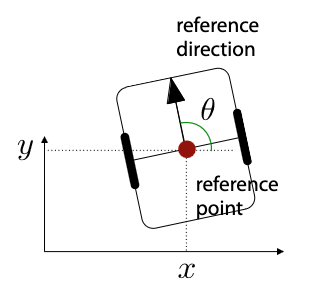
\includegraphics[width=.7\linewidth]{differential}
  %   \caption{$q=(x,y,\theta)$}\label{Fig:Data1}
  % \end{minipage}\hfill
  % \begin{minipage}{0.48\textwidth}
  %   \centering
  %   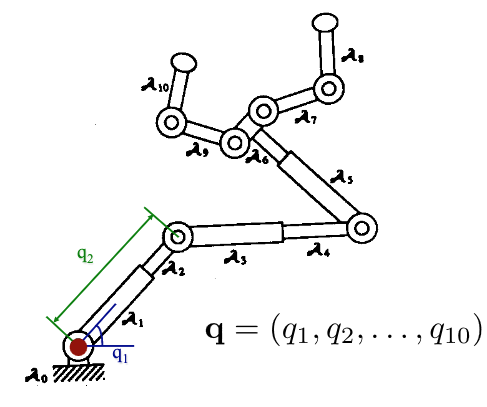
\includegraphics[width=.7\linewidth]{links}
  %   \caption{$q=(q{1},q_{2},...,q_{10})$}\label{Fig:Data2}
  % \end{minipage}
  %\end{figure}

%  \subsection*{Espacio de configuraciones}
  
%\begin{figure}[!htb]
%   \begin{minipage}{0.48\textwidth}
%     \centering
%     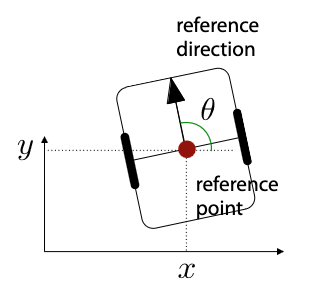
\includegraphics[width=.7\linewidth]{differential}
%     \caption{$q=(x,y,\theta)$}\label{Fig:Data3}
%   \end{minipage}\hfill
%   \begin{minipage}{0.48\textwidth}
%     \centering
%     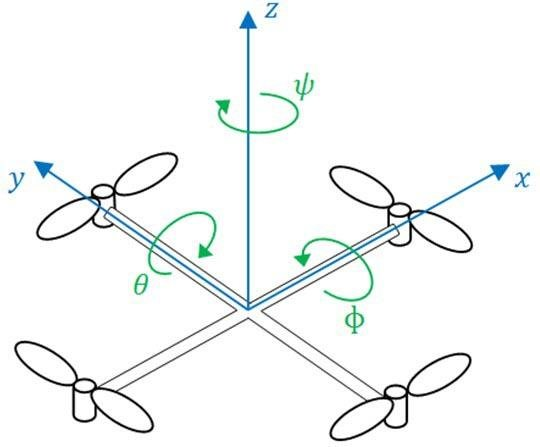
\includegraphics[width=.7\linewidth]{multirotor}
%     \caption{$q=(q{1},q_{2},...,q_{10})$}\label{Fig:Data4}
%   \end{minipage}
%\end{figure}

%Es el espacio de todas las posibles configuraciones, esta compuesto por los espacios libres ($C_{free}$) y espacios ocupado (con obstaculos) $C_{obs}$.\\

%Sea $\mathcal{W} = \mathbb{R}^{m}$, $\mathcal{O} \in \mathcal{W}$ el conjunto de obstaculos, $\mathcal{A}(q)$ las configuraciones del robot $q \in \mathcal{C}$

%\begin{itemize}
%  \item $C_{free} = \{q \in \mathcal{C}|\mathcal{A}(q)\cap\mathcal{O} = \emptyset\}$
%  \item $C_{obs} = C/C_{free}$
%\end{itemize}

%donde $\mathcal{W} = \mathbb{R}^{m}$ es el espacio de trabajo del robot, $\mathcal{O} \in \mathcal{W}$ es el conjunto de obstaculos, y $\mathcal{A}(q)$ son las configuraciones del robot $q \in \mathcal{C}$ .\\

%\st{Com\'{u}nmente se relaciona al problema de planificaci\'{o}n de rutas con el problema del mover un piano (\textbf{piano movement problem}). Es un problema dif\'{i}cil ya que el piano es un objeto en $\mathbb{R}^{3}$ que puede rotar y trasladarse. La \textbf{planificaci\'{o}n de rutas}, es similar. Ya que queremos mover al robot a un punto especifico.}\\

%\st{En problemas cl\'{a}sicos de planificaci\'{o}n de rutas decimos que el camino \'{o}ptimo es el camino m\'{a}s corto, hay distintas formas cualitativas de poder ver un camino corto (Minimizando la energ\'{i}a en la trayectoria ..etc).}\\

%Nuestra soluci\'{o}n se centra en buscar la posible manera m\'{a}s r\'{a}pida de llegar de un punto al otro.\\

La planificaci\'{o}n de rutas presenta diversos retos:
\begin{itemize}
\item Restricciones fisicas del robot (su geometr\'{i}a o forma)
\item Din\'{a}mica del robot
\item Incertidumbres de lecturas de sensores (ruido)
\end{itemize}

Para crear rutas seguras, debemos respetar las restricciones para que el robot pueda ejecutar los movimientos en el mundo real. Los problemas que emergen de la planificaci\'{o}n de trayectorias es la escalabilidad y eficiencia computacional. Considerando mover un VANT en 3D que puede trasladarse y rotar. El problema ser\'{a} en optimizar varios parametros por los 6 DoF (Grados de libertad) que cuenta buscando algoritmos que corran en tiempo real (que se ejecuten r\'{a}pido) dentro de dispositivos computacionales limitados.\\

%\st{Entonces, si le ordenamos al robot que ejecute una acci\'{o}n particular a trav\'{e}s de su interfaz de control, \textquestiondown qu\'{e} tan seguros estaremos de que el robot realmente lleg\'{o} a ese punto sin estar observandolo?}\\


%\st{Considerando mover un VANT en 3D que puede trasladarse y rotar. El problema ser\'{a} en optimizar varios parametros por los 6 DoF (Grados de libertad) que cuenta y si queremos algoritmos que corran en tiempo real (que se ejecuten r\'{a}pido) dentro de dispositivos computacionales limitados.}\\

%Finalmente habr\'{a} obst\'{a}culos o otros robots en el ambiente que nuestra soluci\'{o}n de arquitectura deba considerar en su planificaci\'{o}n. El robot debe sensar los obst\'{a}culos y evitarlos.

%\subsection*{Robots aereos}

%\cite{10120941} clasifican los Veh\'{i}culos A\'{e}reos No Tripulados (VANT) principalmente en tres grups \textbf{Ala Fija, Ala Rotatoria y Hibrido}\\

%UAVs are typically categorized as fixed-wing, rotary-wing, and hybrid-wing. Fixed-wing UAVs have rigid wings, like conventional human aircraft. They require relative velocity to generate aerodynamic forces and are thus more aero-dynamically efficient; however, fixed-wing UAVs require a runway for takeoff and landing. Vertical takeoff and landing are possible for rotary-wing UAVs because their revolving rotary blades generate adequate aerodynamic thrust. \cite{10120941}

%Mostrar la figura 1 de \cite{10120941}, mostrar la figura 2 \cite{10120941}\\
%Mostrar la tabla 5 \cite{10120941}

%Claramente los problemas inherentes al control de vehiculos aereos son diferentes a los que pueda presentar un robot en tierra. Y su control recae en el ajuste de los angulos presentes en los tres ejes (roll, pitch, yaw).\\

%\cite{UAVCIVIL2019}.
%\st{Millones de Veh\'{i}culos A\'{e}reos No Tripulados, o tambi\'{e}n conocidos como drones, han presentado una adopci\'{o}n masiva en diferentes aplicaciones, desde usos civiles (b\'{u}squeda y rescate, monitoreo industrial, vigilancia), hasta aplicaciones militares. La popularidad de los VANT es atribuida a su movilidad.}\\

%\st{La idea de utilizar m\'{u}ltiples robots a\'{e}reos en un sistema coordinado se basa en el comportamiento de los enjambres de animales, como las abejas o los p\'{a}jaros, que trabajan juntos de manera colaborativa para lograr objetivos comunes. Esta inspiraci\'{o}n biol\'{o}gica ha llevado al desarrollo de algoritmos y t\'{e}cnicas para coordinar y controlar m\'{u}ltiples VANT en diferentes aplicaciones.}\\
  
%\st{El inter\'{e}s en la investigaci\'{o}n e inovaci\'{o}n de soluciones con Veh\'{i}culos A\'{e}reos No Tripulados ha crecido exponencialmente en a\~{n}os recientes} \citenum{Daponte2015,UAVPRACTICAL2023,GUPTA2016,VEGETACION2017,ROADS2017}.\\

%\st{En recientes a\~{n}os, dotar a los VANT de inteligencia para explotar la informaci\'{o}n recolectada de sensores a bordo, ha sido y es un \'{a}rea estudiada en rob\'{o}tica m\'{o}vil \'{a}rea (construcci\'{o}n de mapas)}\citenum{SHUKLA2016490}.\\

%\st{Buscando probar diferentes teor\'{i}as de control, convirti\'{e}ndo los problemas t\'{i}picos de control 2D (p\'{e}ndulo inverso fijo) a un ambiente 3D, teniendo m\'{a}s variables a controlar para mantener el equilibrio del p\'{e}ndulo y al mismo tiempo lograr el movimiento y las maniobras deseadas del dron en el espacio tridimensional} \citenum{PENDU2011}.\\
  
%\st{El despliegue r\'{a}pido de robots en situaciones de riesgo, b\'{u}squeda y rescate ha sido un \'{a}rea ampliamente estudiada en la rob\'{o}tica m\'{o}vil. Donde existen concursos DARPA CHALLENGE donde todos los factores como exploraci\'{o}n, planeaci\'{o}n y coordinaci\'{o}n son clave para lograr los objetivos del Reto.}  \citenum{DARPA2022}. %se han aplicado teor\'{i}as de grafos para la obtenci\'{o}n de la mejor ruta. Los comportamientos reactivos son primordiales si pensamos en un agente aut\'{o}nomo.\\ %Esa percepci\'{o}n que podemos tener los seres humanos para reaccionar a ciertos retos. Buscar la manera de crear una arquitectura de software tolerante a fallas, capaz de coordinar m\'{u}ltiples v\'{e}hiculos a\'{e}reos no trupulados a medida que incrementa o disminuye la oferta de VANT(s) disponibles.\\

%\subsection*{Panorama de m\'{e}todos de planificaci\'{o}n}

%Un modelo del entorno nos ayudar\'{a} a conocer sus variables y reducir rutas inecesarias. Los m\'{e}todos para modelar el ambiente se basan en aproximaciones de espacios, espacios libres, descomposicion por celdas, mapas topologicos y m\'{e}todos probabilisticos como el PRM (probabilistic roadmap method).\\

%Dentro del survey Path Planning for the Mobile Robot\citenum{sym10100450} se\~{n}alan que el n\'{u}mero de publicaciones para planificadores de trayectoria, los algoritmos basados en Inteligencia Artificial han ganado terreno como soluciones para planificaci\'{o}n de trayectorias. Esto es en la b\'{u}squeda de la mejor trayectoria respecto a un mapa ya conocido.\\

%Por otra parte el suvey de \cite{PathPlanning2020} se centra en los planificadores de rutas para VANT haciendo tres clasificaciones: T\'{e}cnicas por representacion, t\'{e}cnicas cooperativas y t\'{e}cnicas no cooperativas. Plantean que el problema de planificaci\'{o}n de trayectorias es considerado como un problema de optimizaci\'{o}n de tal modo de obter una soluci\'{o}n factible entre todas las posibles. \textit{No existe un algoritmo exacto que defina una ruta \'{o}ptima}.\\

%Los procesos m\'{a}s comunes para planificaci\'{o}n son:

%\begin{itemize}
%\item Representaci\'{o}n del VANT en un entorno 3D mostrando los obst\'{a}culos y el espacio libre.
%\item Creaci\'{o}n del mapa o grafo que considere la configuraci\'{o}n y especificaciones del VANT en un entorno 3D.
%\end{itemize}

\cite{XU2023110164}[\citenum{XU2023110164}] mencionan que la planificaci\'{o}n de trayectorias para m\'{u}ltiples VANTS es inherente a lo complejo del entorno y los trayectorias que pueda tomar el VANT. La minimizaci\'{o}n de la longitud de las rutas, configuraciones que pueda realizar el VANT y la seguridad del trayecto para todos los multi-VANT durante el vuelo son partes clave cuando se crea un planificador multi-VANT. Apesar de las aproximaciones los planificadores globales se deben descomponer para poder considerar la existencia de obst\'{a}culos haciendo que la comunicaci\'{o}n entre ellos pueda ser afectada. En \'{u}ltimas decadas se han propuesto diversas t\'{e}cnicas de programaci\'{o}n (Mixed Integer Linear Programming (MILP), Nonlinear programming (NP) y Dynamic Programming (DP)) teniendo estos m\'{e}todos una fuerte base en teor\'{i}a matem\'{a}tica. A pesar de ello estos metodos de programacion matem\'{a}tica su escala computacional crece exponencialmente conforme el espacio de b\'{u}squeda.\\ 
%Tomando como ejemplo uno de sus deseables usos aut\'{o}nomos para b\'{u}squeda y rescate, supongamos que un VANT encuentra el objetivo, informa a los dem\'{a}s VANT para que vengan a ayudar lo m\'{a}s r\'{a}pido posible, la comunicaci\'{o}n entre ellos no debe perderse para lograr completar la tarea.\\
%Es por ello que el conocimiento de algoritmos capaces de planear rutas cooperativas debe ser considerados.\\

Otros m\'{e}todos que han sido ampliamente trabajados son los de Campo de Potencial Artificial ampliamente usado como planificador de trayectorias por sus ventajas en tiempo real. Desafortunadamente cuando existen dos campos de repulsi\'{o}n causados por obst\'{a}culos son iguales, \'{e}ste m\'{e}todo cae en m\'{i}nimos locales llegando a fallar en encontrar una soluci\'{o}n.\\

%Tambien se han propuesto los algoritmos basados en grafos para resolver el problema de planificaci\'{o}n de trayectorias.\\
%Diagramas de Voronoi y el algoritmo A* siguen demostrando en encontrar efectivamente una ruta dependiendo de la division del espacio de busqueda. Estos metodos basados en grafos que funcionan muy bien en ambientes representados en 2D, pero al aplicarse a 3D toman mucho tiempo de ejecucion cuando el espacio de busqueda es complejo \citenum{DENG2023}.\\

Diversas t\'{e}cnicas de Inteligencia Computacional se han propuesto para el problema de planificaci\'{o}n de trayectorias (Algoritmos Gen\'{e}ticos GA, Ant Colony Optimization (ACO) \cite{ZHAO2020} [\citenum{ZHAO2020}], Particle Swarm Optimization (PSO) y Evolucion Diferencial (DE). Estos algoritmos han demostrado crear rutas navegables para los VANT y son apliamente usados para problemas de planificacion de rutas complejos. Trabajos de \cite{DENG2023} [\citenum{DENG2023}] han realizado adaptaciones al algoritmo PSO mostrado mejores resultados evitando caer en m\'{i}nimos locales con ayuda de Algoritmos Gen\'{e}ticos (GA) considerando par\'{a}metros como inercia, funciones de activaci\'{o}n para la probabilidad de cruza y mutaci\'{o}n, mostrando mejorar a rutas r\'{a}pidas y estables en una ejecuci\'{o}n off-line.\\

%\begin{itemize}
%  \item Geom\'{e}tricos
%    \begin{itemize}
%    \item Grafos de visibilidad, descomposici\'{o}n en celdas, diagramas de voronoi, etc.
%    \end{itemize}
%  \item Campos de potencial
%    \begin{itemize}
%    \item Frentes de onta, funciones de navegaci\'{o}n, etc.
%    \end{itemize}
%  \item Basados en b\'{u}squeda
%    \begin{itemize}
%    \item Dijkstra, A*, D*, D* Lite, etc.
%    \end{itemize}
%  \item Basados en pruebas
%    \begin{itemize}
%    \item RRT, RRT*, PRM, etc.
%    \end{itemize}
%  \item Trayectorias
%    \begin{itemize}
%    \item M\'{i}nimo tiempo/energia, etc.
%    \end{itemize}
%  \item Bioinspirados
%    \begin{itemize}
%    \item Redes Neuronales, Algoritmos Geneticos, Ant Colony Optimisation, etc.
%    \end{itemize}
%\end{itemize}

%La siguiente tabla muestra los m\'{e}todos de planificaci\'{o}n de trayectorias.\\



%%%%%%%%%%%%%%%%%%%%%%%%%%%
% IMAGEN Sistema autonomo
%%%%%%%%%%%%%%%%%%%%%%%%%%%

%\begin{itemize}
%\item Hablar de la robotica de servicios
%\item robotica movil
%\item clasificar los diversos robots moviles aereos
%\item los problemas en la robotica movil
%\item slam
%\item robots coolaborativos
%\end{itemize}

%%%%%%%%%%%%%%%%%%%%%%%%%%%

%%%%%%%%%%%%%%%%%%%%%%%%%%%

%\noindent\makebox[\linewidth]{\rule{\paperwidth}{0.4pt}}

%\begin{center}
%\fbox{\parbox[t]{14em}{
%    \begin{itemize}
%      \tiny \item Caracteristicas Robot
%      \begin{itemize}
%        \tiny \item Grados de libertad
%        \tiny \item Fisica del robot
%        \tiny \item limitaciones en Mobilidad
%        \tiny \item limitaciones en Dinamica
%      \end{itemize}
%    \end{itemize}
%  }
%}%
%\raisebox{-10ex}{\Huge$\to$}%
%\fbox{\parbox[t]{14em}{
%    \begin{itemize}
%      \tiny \item Propiedades del algortimo
%      \begin{itemize}
%        \tiny \item Optimalidad
%        \tiny \item Costo Computacional
%        \tiny \item Costo en memoria
%        \tiny \item Completez
%        \tiny \item Online vs. Offline
%        \tiny \item Anytime
%        \tiny \item Caminos vs. trayectorias
%        \tiny \item Exactos vs. aproximados
        
%      \end{itemize}
%    \end{itemize}
%  }
%}
%\end{center}

\begin{figure}
  \begin{center}
    \begin{forest}
      for tree={%
        thick,
        drop shadow,
        l sep=0.6cm,
        s sep=0.8cm,
        node options={draw,font=\sffamily},
        edge={semithick,-Latex},
        where level=0{parent}{},
        where level=1{
          minimum height=1cm,
          child,
          parent anchor=south west,
          tier=p,
          l sep=0.25cm,
          for descendants={%
            grandchild,
            minimum height=0.6cm,
            anchor=250,
            edge path={
              \noexpand\path[\forestoption{edge}]
              (!to tier=p.parent anchor) |-(.child anchor)\forestoption{edge label};
            },
          }
        }{},
      }
      [Retos\\multi-VANT, draw=black, top color=white!5, bottom color=white!30
        [Planificaci\'{o}n\\trayectorias, draw=gray!30, top color=gray!5, bottom color=gray!30
          [Creaci�n de formaciones\\, draw=gray!10, top color=gray!5, bottom color=gray!10
            [Evasi\'{o}n \\de obst\'{a}culos, draw=gray!10, top color=gray!5, bottom color=gray!10
              [M\'{u}ltiples objetivos, draw=gray!10, top color=gray!5, bottom color=gray!10]
            ]
          ]
        ]
        [Percepci\'{o}n, draw=gray!30, top color=gray!5, bottom color=gray!30
          [Colecci\'{o}n de\\informaci\'{o}n, draw=gray!10, top color=gray!5, bottom color=gray!10
            [An\'{a}lisis de im\'{a}genes, draw=gray!10, top color=gray!5, bottom color=gray!10
              [Construcci\'{o}n de mapas, draw=gray!10, top color=gray!5, bottom color=gray!10]
            ]
          ]
        ]
        [Comunicaci\'{o}n, draw=gray!30, top color=gray!5, bottom color=gray!30
          [Conectividad entre agentes, draw=gray!10, top color=gray!5, bottom color=gray!10
            [Tolerable a fallos, draw=gray!10, top color=gray!5, bottom color=gray!10
              [Seguridad de datos, draw=gray!10, top color=gray!5, bottom color=gray!10]
            ]
          ]
        ]
        [Control de Vuelo, draw=gray!30, top color=gray!5, bottom color=gray!30
          [Controles tipo PID, draw=gray!10, top color=gray!5, bottom color=gray!10
            [M\'{e}todos \\basados en aprendizaje, draw=gray!10, top color=gray!5, bottom color=gray!10
              [Controles\\lineales de vuelo, draw=gray!10, top color=gray!5, bottom color=gray!10]
            ]
          ]
        ]
      ]
    \end{forest}
  \end{center}
  \caption{Ilustra los retos multi-VANT}\label{fig:retos}
\end{figure}


\newpage
\section*{Planteamiento del problema}

Desarrollar una estrategia de exploraci\'{o}n multi-VANT que reduzca el tiempo total de exploraci\'{o}n dado un conjunto de $\mathcal{V}$ veh\'{i}culos a\'{e}reos no tripulados. Las capacidades limitadas de energ\'{i}a y sensores abordo de los VANT les permiten navegar de forma aut\'{o}noma. Teniendo en cuenta sus limitaciones de energ\'{i}a y la necesidad de una exploraci\'{o}n eficiente, el objetivo es determinar la trayectoria, las rutas y la asignaci\'{o}n de tareas \'{o}ptimas.\\

El espacio de todas las posibles configuraciones, est\'{a} compuesto por los espacios libres ($C_{free}$) y espacios ocupado (con obst\'{a}culos) $C_{obs}$.\\

Sea $\mathcal{W} = \mathbb{R}^{3}$ el mundo, $\mathcal{O} \in \mathcal{W}$ el conjunto de obst\'{a}culos,\\
$\mathcal{A}(q)$ las configuraciones del robot $q \in \mathcal{C}$

\begin{itemize}
  \item $C_{free} = \{q \in \mathcal{C} | \mathcal{A}(q)\cap\mathcal{O} = \emptyset\}$
  \item $C_{obs} = C \setminus C_{free}$
\end{itemize}

donde $\mathcal{W} = \mathbb{R}^{3}$ es el espacio de trabajo del robot, $\mathcal{O} \in \mathcal{W}$ es el conjunto de obst\'{a}culos, y $\mathcal{A}(q)$ son las configuraciones del robot $q \in \mathcal{C}$ .\\

%Com\'{u}nmente se relaciona al problema de planificaci\'{o}n de rutas con el problema del mover un piano (\textbf{piano movement problem}). Es un problema dif\'{i}cil ya que el piano es un objeto en $\mathbb{R}^{3}$ que puede rotar y trasladarse. La \textbf{planificaci\'{o}n de rutas}, es similar. Ya que queremos mover al robot a un punto especifico.\\

%\textquestiondown Qu\'{e} acciones deber\'{a} realizar el VANT para explorar el espacio completo lo m\'{a}s r\'{a}pido posible?.\\

La soluci\'{o}n debe tener en cuenta los obst\'{a}culos, los entornos din\'{a}micos, las limitaciones de comunicaci\'{o}n y la coordinaci\'{o}n entre los VANTS para evitar colisiones. Para lograr una exploraci\'{o}n eficiente y completa con un tiempo y recursos m\'{i}nimos, el problema requiere la creaci\'{o}n de algoritmos y t\'{e}cnicas de optimizaci\'{o}n.\\

Completar la exploraci\'{o}n significa que el robot pueda crear un mapa $\mathcal{M}$ que cubre el volumen $\mathcal{V}$ y los puntos en el mapa. Por la naturaleza del problema, esto se debe resolver de forma r\'{a}pida sin tiempos de espera.\\

%La coordinaci\'{o}n de m\'{u}ltiples-VANT (Veh\'{i}culos A\'{e}reos No Tripulados) es un desaf\'{i}o complejo en el campo de la rob\'{o}tica y la exploraci\'{o}n de \'{a}reas desconocidas. A medida que la tecnolog\'{i}a de los Veh\'{i}culos A\'{e}reos No Tripulados contin\'{u}a avanzando y se vuelven m\'{a}s accesibles, se presenta la oportunidad de utilizar equipos de m\'{u}ltiples VANT para realizar tareas de manera colaborativa y eficiente. Sin embargo, esta coordinaci\'{o}n planea diversas problem\'{a}ticas que deben abordarse.\\

%\st{La coordinaci\'{o}n de m\'{u}ltiples VANT implica la necesidad de establecer una comunicaci\'{o}n efectiva entre ellos. Los VANT deben intercambiar informaci\'{o}n relevante sobre su posici\'{o}n, estado, objetivos y otros datos importantes. La comunicaci\'{o}n debe ser confiable, de baja latencia y capaz de manejar m\'{u}ltiples enlaces de manera simult\'{a}nea.}\\

%Otro desaf\'{i}o es la planificaci\'{o}n de rutas y la toma de decisiones distribuida. Los VANT deben coordinar sus movimientos para evitar colisiones y lograr una cobertura eficiente del \'{a}rea objetivo. Esto implica la necesidad de desarrollar algoritmos y estrategias que permitan la planificaci\'{o}n de rutas din\'{a}micas, considerando los obst\'{a}culos y las restricciones del entorno. Adem\'{a}s, los VANT deben tomar decisiones colaborativas para adaptarse a situaciones imprevistas o cambios en el entorno.\\

%La asignaci\'{o}n de tareas tambi\'{e}n es un aspecto cr\'{i}tico en la coordinaci\'{o}n de m\'{u}ltiples VANT. Cada VANT puede tener diferentes capacidades y sensores especializados, por lo que es importante asignar tareas de acuerdo con las fortalezas individuales de cada robot. Adem\'{a}s, los VANT deben colaborar en la recolecci\'{o}n y procesamiento de datos, evitanto la duplicaci\'{o}n de esfuerzos optimizando el uso de los recursos disponibles.\\

%\st{Dada un \'{a}rea de inter\'{e}s $A$ desconocida que se desea explorar,}

%\begin{itemize}
%\item \st{Un conjunto de Veh\'{i}culos A\'{e}reos No Tripulados (VANT) denotados como $V = \{V_{1},V_{2},V_{3},...,V_{n}\}$, donde $n$ es el n\'{u}mero total de VANT's disponibles}
%\item \st{Un conjunto de tareas de exploraci\'{o}n denotados como $T = \{T_{1}, T_{2}, T_{3}, T_{m}\}$, donde $m$ es el n\'{u}mero total de tareas a realizar.}
%\end{itemize}

%\st{restricciones y requisitos espec\'{i}ficos del problema, como l\'{i}mites de tiempo, obst\'{a}culos a evitar. Para cada tarea de exploraci\'{o}n $T_{m}$, se definen las siguientes variables:}

%\begin{itemize}
%\item \st{Posici\'{o}n inicial: $p_{i}(x,y,z)$, representa la posici\'{o}n inicial del VANT o los m\'{u}ltiples-VANTs asignados a la tarea $T_{m}$}
%\item \st{Trayectoria: $\alpha_{i}$, describe la trayectoria seguida por el/los VANT asignado(s) a la tarea $T_{m}$ en funci\'{o}n del tiempo $t$}
%\item \st{Informaci\'{o}n recolectada: $C_{i}$, representa la informaci\'{o}n recolectada por el/los VANT asignado(s) durante la exploraci\'{o}n}
%\end{itemize}

La funci\'{o}n objetivo variar\'{a} seg\'{u}n los objetivos espec\'{i}ficos del problema.
\begin{itemize}
\item Maximizar la cobertura del \'{a}rea de inter\'{e}s $C$
\item Minimizar el tiempo total requerido para cubrir el \'{a}rea de inter\'{e}s $C$
\item Maximizar la cantidad de informaci\'{o}n recolectada
\end{itemize}

Con base en lo anterior, surgen las siguientes preguntas de investigaci\'{o}n:
\begin{itemize}
\item \textquestiondown Qu\'{e} acciones deber\'{a}n de realizar los VANTS para explorar el espacio completo lo m\'{a}s r\'{a}pido posible?
\item \textquestiondown Cual\'{e}s son los mejores algoritmos adecuados para correr en una tarjeta electr\'{o}nica con recursos limitados?
\item \textquestiondown Qu\'{e} tan seguros estaremos que un nuevo VANT a la misi\'{o}n llegue a la frontera y aporte a la misi\'{o}n?
\end{itemize}

\subsection*{Hip\'{o}tesis}

%Es posible crear una arquitectura de software para coordinar m\'{u}ltiples-VANTS para tareas de exploraci\'{o}n capaz de contar con una representacion del ambiente en voxels.
La eficiencia de exploraci\'{o}n y la cobertura de un \'{a}rea objetivo se pueden mejorar empleando un enfoque coordinado, colaborativo y descentralizado. El sistema multi-VANT puede lograr una exploraci\'{o}n m\'{a}s completa a trav\'{e}s de la asignaci\'{o}n efectiva de tareas, la planificaci\'{o}n de la trayectoria y la coordinaci\'{o}n. La hip\'{o}tesis asume que la integraci\'{o}n de m\'{u}ltiples VANTS con diversas capacidades conducir\'{a} a mejores resultados de exploraci\'{o}n, incluida una mayor cobertura de \'{a}rea, una mejor recopilaci\'{o}n de datos y un rendimiento general mejorado en comparaci\'{o}n con un enfoque de un solo VANT.

\section*{Objetivos generales y espec\'{\i}ficos del proyecto}

\textbf{General} \\

Dise\~{n}ar una arquitectura de software descentralizada capaz de resolver los problemas de localizaci\'{o}n, mapeo, navegaci\'{o}n y coordinaci\'{o}n multi-VANT en ambientes desconocidos y din\'{a}micos para tareas de exploraci\'{o}n en interiores.

%Desarrollo e implementaci\'{o}n de una arquitectura de software tolerante a fallas para la coordinaci\'{o}n de m\'{u}ltiples VANT(s) aplicados a una simulaci\'{o}n de b\'{u}squeda y rescate.

%El objetivo general de la tesis es desarrollar estrategias efectivas para la coordinación de m\'{u}ltiples Veh\'{i}culos A\'{e}reos no Tripulados, con el fin de mejorar la eficiencia y el rendimiento en aplicaciones en exploraciones aéreas.

\bigskip
\noindent
%\textbf{Particulares} \\
De manera m\'{a}s espec\'{i}fica, se listan los siguientes objetivos: %espec\'{i}ficos:

\begin{enumerate}

\item \textbf{Construcci\'{o}n propuesta} Evaluar las soluciones en la literatura asociados con la coordinaci\'{o}n multi-VANT. Enfoc\'{a}ndose en aspectos como la comunicaci\'{o}n, evasi\'{o}n de obst\'{a}culos, asignaci\'{o}n de tareas y sincronizaci\'{o}n de informaci\'{o}n. Bas\'{a}ndose a esta valoraci\'{o}n, construir una arquitectura de software para la coordinaci\'{o}n multi-VANT.

\item \textbf{Valoraci\'{o}n (prueba) propuesta} Emplear una herramienta de simulaci\'{o}n de libre uso para rob\'{o}tica, para el desarrollo y puesta en marcha de una propuesta de arquitectura de software capaz de realizar el control multi-VANT y evaluar el desemple\~{n}o de dicha arquitectura.
  
\item \textbf{Comparaci\'{o}n y an\'{a}lisis} Comparar y analizar los resultados obtenidos con enfoques existentes en la coordinaci\'{o}n multi-VANT, mostrando las ventajas y desventajas de la estrategia propuesta. Con base a estos an\'{a}lisis proponer recomendaciones y pautas pr\'{a}cticas para la implementaci\'{o}n y aplicaci\'{o}n de la estrategias de coordinaci\'{o}n multi-VANT en escenarios reales, considerando factores como la escalabilidad, la robustez y los recursos computacionales requeridos.

\end{enumerate}

\section*{Metodolog\'{\i}a}

La metodolog\'{i}a propuesta se divide en tres etapas, iniciando en septiembre del 2023 y terminando en agosto del 2024. A continuaci\'{o}n se detallan cada una de las actividades que se plantean realizar en cada una.

\subsection*{Etapa 1. An\'{a}lisis y dise\~{n}o de la soluci\'{o}n propuesta}

En esta etapa se comprende en la revisi\'{o}n de la literatura de manera m\'{a}s completa, que permita contar con la informaci\'{o}n necesaria para la elecci\'{o}n de los mejores algoritmos para abordar cada una de las problem\'{a}ticas asociadas con la coordinaci\'{o}n de trayectorias. Una vez realizada la elecci\'{o}n de los algoritmos que se usar\'{a}n para la propuesta de arquitectura de software, se proceder\'{a} a revisar y estudiar las arquitecturas para los robots colaborativos. Finalmente, se realizar\'{a} el dise\~{n}o de la arquitectura.\\

Las actividades espec\'{i}ficas a realizarse en la etapa 1, son:
  
  \begin{enumerate}
  \item[] \textbf{E1.A1.} \textbf{Revisi\'{o}n estado del arte} Ampliar la revisi\'{o}n de la literatura sobre coordinaci\'{o}n y exploraci\'{o}n multi-VANT.
  \item[] \textbf{E1.A2.} \textbf{Evaluaci\'{o}n de aptitudes} Revisar y documentar los aspectos relevantes (asi como sus limitantes) que permiten la colaboraci\'{o}n, coordinaci\'{o}n y balanceo de la carga de trabajo multi-VANT.
  %\item \textbf{E1.A3.} \textbf{Selecci\'{o}n de algoritmos} Estudiar las limitantes de las soluciones relevantes en la literatura en base a autonomia e inteligencia computacional.
  \item[] \textbf{E1.A3.} \textbf{Selecci\'{o}n de algoritmos} Seleccionar los algoritmos para planificaci\'{o}n de trayectorias y exploraci\'{o}n en ambientes desconocidos representativos para un entorno de computaci\'{o}n restringida.
  \item[] \textbf{E1.A4.} \textbf{Elaboraci\'{o}n de soluci\'{o}n} Definir la arquitectura de software para escenarios en aplicaciones multi-VANT apegadas a las especificaciones de computadora de placa reducida (Raspberry Pi, Esp32 ... etc.).
  \item[] \textbf{E1.A5.} \textbf{Documentaci\'{o}n Etapa 1} Elaborar la documentaci\'{o}n de la revisi\'{o}n del estado del arte y del trabajo realizado que formar\'{a} parte de la tesis.
  \item[] \textbf{E1.A6.} \textbf{Revisi\'{o}n de tesis Etapa 1} Revisi\'{o}n y correcci\'{o}n de avances con los asesores.
  \end{enumerate}
  
  \subsection*{Etapa 2. Implementaci\'{o}n y validaci\'{o}n}
  
  Esta etapa se centra en el desarrollo e implementaci\'{o}n del dise\~{n}o de la arquitectura de software para la coordinaci\'{o}n multi-VANT.\\
  
  Las actividades espec\'{i}ficas a realizarse en la etapa 2, son:

  \begin{enumerate}
  \item[] \textbf{E2.A1.} \textbf{Selecci\'{o}n Simulador} Al tener definida la arquitectura de software y conocer las estructuras de datos que se utilizaran, evaluar los diversos simuladores para rob\'{o}tica de libre uso. (Revisar temas de modelos 3D, din\'{a}mica del robot, representaci\'{o}n del ambiente 3D, simulaci\'{o}n de sensores). 
  \item[] \textbf{E2.A2.} \textbf{Visualizaci\'{o}n de datos} Conocer las herramientas para la visualizaci\'{o}n y telemetr\'{i}a y creaci\'{o}n de un modelo 3D de acuerdo al simulador seleccionado.
  \item[] \textbf{E2.A3.} \textbf{Control de desplazamientos} Crear movimientos y control de un VANT y m\'{u}ltiples VANTS, algoritmos que forman parte de la capa reactiva del VANT.
  %\item[] \textbf{E2.A4.} \textbf{Desarrollo de visualizaci\'{o}n de datos} A partir de la selecci\'{o}n del sensor, se desarrollar\'{a} la forma de representar el entorno 3D dentro del simulador elegido.
  \item[] \textbf{E2.A4.} \textbf{Desarrollo de algoritmos de exploraci\'{o}n} De acuerdo con la revisi\'{o}n del estado del arte se implementar\'{a} el algoritmo propuesto para la exploraci\'{o}n con un VANT
  \item[] \textbf{E2.A5.} \textbf{Implementaci\'{o}n un solo VANT} Realizar pruebas y corregir errores con base a los desarrollos realizados.
  \item[] \textbf{E2.A6.} \textbf{Simulaci\'{o}n un solo VANT} Realizar pruebas de simulaci\'{o}n con un solo VANT de la soluci\'{o}n propuesta.
  \item[] \textbf{E2.A7.} \textbf{Desarrollo de coordinaci\'{o}n} Al contar con la exploraci\'{o}n y navegaci\'{o}n exitosa de un solo VANT, se procede al desarrollo de coordinaci\'{o}n multi-VANT.
  \item[] \textbf{E2.A8.} \textbf{Implementaci\'{o}n multi-VANT} Realizar pruebas y correcci\'{o}n de errores con base a los desarrollos realizados para la coordinaci\'{o}n multi-VANT.
  \item[] \textbf{E2.A9.} \textbf{Simulaci\'{o}n multi-VANT} Realizar pruebas de simulaci\'{o}n multi-VANT de la soluci\'{o}n propuesta.
  \item[] \textbf{E2.A10.} \textbf{Documentaci\'{o}n Etapa 2} Elaborar la documentaci\'{o}n del desarrollo e implementaci\'{o}n de la propuesta de arquitectura de software para la coordinaci\'{o}n multi-VANT que formar\'{a} parte de la tesis.
  \item[] \textbf{E2.A11.} \textbf{Revisi\'{o}n de tesis Etapa 2} Revisi\'{o}n y correcci\'{o}n de cap\'{i}tulos con los asesores.
  \end{enumerate}
  

  \subsection*{Etapa 3. Evaluaci\'{o}n experimental, resultados y conclusiones}
  
  Partiendo del prototipo y las simulaciones desarrolladas en la etapa anterior, en esta etapa se realizan todas las actividades relacionadas con la evaluacion, recabacion de resultados y la escritura de los capitulos restantes de la tesis. Ademas se realizara el proceso de graduacion y actividades relacionadas.\\

  Las actividades espec\'{i}ficas a realizarse en la etapa 3, son:
  
  \begin{enumerate}
  \item[] \textbf{E3.A1.} \textbf{Experimentaci\'{o}n de soluci\'{o}n} Experimentos para evaluar el desempe\~{n}o de la solucion propuesta creada en la etapa anterior.  
  \item[] \textbf{E3.A2.} \textbf{Recopilaci\'{o}n de resultados} Recabar la informacion de los resultados, realizar su analisis y generar la documentacion correspondiente.
  \item[] \textbf{E3.A3.} \textbf{Documentaci\'{o}n Etapa 3} Elaborar la documentaci\'{o}n de los resultados obtenidos y conclusiones que formar\'{a} parte de la tesis.
  \item[] \textbf{E3.A4.} \textbf{Revisi\'{o}n de tesis} Revisi\'{o}n y correcci\'{o}n de tesis con los asesores.
  \item[] \textbf{E3.A5.} \textbf{Divulgaci\'{o}n} De acuerdo a los progresos dentro de la tesis, se estar\'{a} en total disposici\'{o}n a espacios donde se pueda hacer divulgaci\'{o}n cient\'{i}fica dentro del estado cubriendo los requisitos de retribuci\'{o}n social de la instituci\'{o}n.
  \item[] \textbf{E3.A6.} \textbf{Proceso de titulaci\'{o}n} Comenzar el proceso de titulaci\'{o}n.
  \end{enumerate}

  \section*{Infraestructura}
  
  Para el desarrollo de este proyecto de investigaci\'{o}n, se har\'{a} uso de un equipo de c\'{o}mputo con las siguientes caracter\'{i}sticas:
  
  \begin{itemize}
  \item iMac (21.5-inch, Late 2015)
  \item Procesador 2.8 GHz Quad-Core Intel Core i5
  \item Memoria Ram 8 GB 1867 MHz DDR3
  \item Graphics Intel Iris Pro Graphics 6200 1536 MB
  \item Almacenamiento 1 TB
  \end{itemize}
  
  
  
\section*{Cronograma de actividades (plan de trabajo)}

\hspace{-1.4cm}\begin{minipage}{10cm}
\noindent\begin{tabular}{|p{0.8\textwidth}*{12}{|p{0.040\textwidth}}|}
% The top line
%\diagbox[width=12.5em]{Actividades}{Cuatrimestres}
\hline
& \multicolumn{4}{c|}{\textbf{Cuatrimestre 1\footnote{Correspondiente a los meses de Septiembre, Octubre, Noviembre, Diciembre del 2023}}} 
& \multicolumn{4}{c|}{\textbf{Cuatrimestre 2\footnote{Correspondiente a los meses de Enero, Febrero, Marzo, Abril del 2024}}}   
& \multicolumn{4}{c|}{\textbf{Cuatrimestre 3\footnote{Correspondiente a los meses de Mayo, Junio, Julio, Agosto del 2024}}}\\
\hline
% The second line, with its five years of four quarters
%\textcolor{black}{\textbf{Etapas}}
\rpt[3]{& 1 & 2 & 3 & 4} \\
\hline
\rowcolor{black!5}{\textbf{Etapa 1}}\\
% using the on macro to fill in twenty cells as `on'
%\specialcell{Actividad 1\\espacio}        \on[0] \off[12] \\
%Actividad 1    \on[0] \off[12]\\
\hline
\textbf{E1.A1.} Revisi\'{o}n literatura relevante\footnote{Revisi\'{o}n de alertas de trabajos relacionados sobre la exploraci\'{o}n y colaboraci\'{o}n multi-VANT, evaluaci\'{o}n de aptitudes en trabajos recientes}
%en exploraci\'{o}n multi-VANT, estrategias de exploraci\'{o}n, algoritmos de coordinaci\'{o}n y evaci\'{o}n de obst\'{a}culos
\on[12] \\
\hline
%\textbf{E1.A2.} Evaluaci\'{o}n de aptitudes\footnote{Evaluaci\'{o}n a partir de los nuevos trabajos}     \on[12] \\
%\hline
\textbf{E1.A2.} Selecci\'{o}n de algoritmos \on[2] \off[10] \\
\hline
\textbf{E1.A3.} Dise\~{n}o de la arquitectura de software \off[1] \on[3] \off[8] \\
\hline
\textbf{E1.A4.} Documentaci\'{o}n Etapa 1 \on[4]  \off[8] \\
\hline
\textbf{E1.A5.} Revisi\'{o}n de tesis Etapa 1 \off[3] \on[1]  \off[8] \\
\hline
% using the on macro followed by the off macro
\rowcolor{black!5}{\textbf{Etapa 2}}\\
\hline
\textbf{E2.A1.} Selecci\'{o}n Simulador
\on[1]  \off[11] \\
\hline
\textbf{E2.A2.} Visualizaci\'{o}n de datos\footnote{Visualizaci\'{o}n Octomap en Simulador}
\off[1] \on[2]  \off[9] \\
\hline
\textbf{E2.A3.} Control de desplazamientos\footnote{Un VANT}
\off[2] \on[2]  \off[8] \\
\hline
\textbf{E2.A4.} Desarrollo de algoritmo de exploraci\'{o}n
\off[3] \on[2] \off[7] \\
\hline
\textbf{E2.A5.} Implementaci\'{o}n y simulaci\'{o}n\footnote{Se considera un solo agente que resuelva la tarea de exploraci\'{o}n aut\'{o}noma con evaci\'{o}n de obst\'{a}culos}
\off[3] \on[2] \off[7] \\
\hline
%\textbf{E2.A6.} Simulaci\'{o}n un solo VANT
%\off[4] \on[1] \off[7] \\
%\hline
\textbf{E2.A6.} Desarrollo de coordinaci\'{o}n
\off[4] \on[3] \off[5] \\
\hline
\textbf{E2.A7.} Implementaci\'{o}n y sumulaci\'{o}n\footnote{Se consider\'{a}n los m\'{u}ltiples-VANT que resuelva la tarea de exploraci\'{o}n aut\'{o}noma con evaci\'{o}n de obst\'{a}culos}
\off[6] \on[2] \off[4] \\
\hline
%\textbf{E2.A9.} Simulaci\'{o}n multi-VANT
%\off[6] \on[1] \off[5] \\
%\hline
\textbf{E2.A8.} Documentaci\'{o}n Etapa 2
\off[4] \on[4] \off[4] \\
\hline
\textbf{E2.A9.} Revisi\'{o}n de tesis Etapa 2
\off[7] \on[1] \off[4] \\
\hline
\rowcolor{black!5}{\textbf{Etapa 3}}\\
\hline
\textbf{E3.A1.} Experimentaci\'{o}n de soluci\'{o}n
\off[7]  \on[3] \off[2] \\
\hline
\textbf{E3.A2.} Recopilaci\'{o}n resultados
\off[9]  \on[1] \off[2] \\
\hline
\textbf{E3.A3.} Documentaci\'{o}n Etapa 3
\off[8] \on[3] \off[1] \\
\hline
\textbf{E3.A4.} Revisi\'{o}n de tesis
\off[10] \on[2] \\
\hline
\textbf{E3.A5.} Divulgaci\'{o}n\footnote{Abierto a espacios de divulgaci\'{o}n de acuerdo con las actividades de retribuci\'{o}n social}
\off[5]  \on[7] \\
\hline
\textbf{E3.A6.} Proceso de titulaci\'{o}n
\off[11] \on\\
\hline
\end{tabular}
\end{minipage}

\iffalse
\begin{ganttchart}[vgrid={draw=none, dotted}]{1}{12}
\gantttitlelist{1,...,12}{1} \\
\ganttbar{}{1}{4} \\
\ganttbar{}{5}{11}
\end{ganttchart}


\definecolor{barblue}{RGB}{153,204,254}
\definecolor{groupblue}{RGB}{51,102,254}
\definecolor{linkred}{RGB}{165,0,33}
\renewcommand\sfdefault{phv}
\renewcommand\mddefault{mc}
\renewcommand\bfdefault{bc}

\setganttlinklabel{s-s}{START-TO-START}
\setganttlinklabel{f-s}{FINISH-TO-START}
\setganttlinklabel{f-f}{FINISH-TO-FINISH}
\sffamily
\begin{ganttchart}[
    canvas/.append style={fill=none, draw=black!5, line width=.75pt},
    hgrid style/.style={draw=black!5, line width=.75pt},
    vgrid={*1{draw=black!5, line width=.75pt}},
    today=7,
    today rule/.style={
      draw=black!64,
      dash pattern=on 3.5pt off 4.5pt,
      line width=1.5pt
    },
    today label font=\small\bfseries,
    title/.style={draw=none, fill=none},
    title label font=\bfseries\footnotesize,
    title label node/.append style={below=7pt},
    include title in canvas=false,
    bar label font=\mdseries\small\color{black!70},
    bar label node/.append style={left=2cm},
    bar/.append style={draw=none, fill=black!63},
    bar incomplete/.append style={fill=barblue},
    bar progress label font=\mdseries\footnotesize\color{black!70},
    group incomplete/.append style={fill=groupblue},
    group left shift=0,
    group right shift=0,
    group height=.5,
    group peaks tip position=0,
    group label node/.append style={left=.6cm},
    group progress label font=\bfseries\small,
    link/.style={-latex, line width=1.5pt, linkred},
    link label font=\scriptsize\bfseries,
    link label node/.append style={below left=-2pt and 0pt}
  ]{1}{13}
  \gantttitle[
    title label node/.append style={below left=7pt and -3pt}
  ]{CUATRIMESTRE:\quad1}{1}
  \gantttitlelist{2,...,13}{1} \\
  \ganttgroup[progress=57]{WBS 1 Summary Element 1}{1}{10} \\
  \ganttbar[
    progress=75,
    name=WBS1A
  ]{\textbf{WBS 1.1} Activity A}{1}{8} \\
  \ganttbar[
    progress=67,
    name=WBS1B
  ]{\textbf{WBS 1.2} Activity B}{1}{3} \\
  \ganttbar[
    progress=50,
    name=WBS1C
  ]{\textbf{WBS 1.3} Activity C}{4}{10} \\
  \ganttbar[
    progress=0,
    name=WBS1D
  ]{\textbf{WBS 1.4} Activity D}{4}{10} \\[grid]
  \ganttgroup[progress=0]{WBS 2 Summary Element 2}{4}{10} \\
  \ganttbar[progress=0]{\textbf{WBS 2.1} Activity E}{4}{5} \\
  \ganttbar[progress=0]{\textbf{WBS 2.2} Activity F}{6}{8} \\
  \ganttbar[progress=0]{\textbf{WBS 2.3} Activity G}{9}{10}
  \ganttlink[link type=s-s]{WBS1A}{WBS1B}
  \ganttlink[link type=f-s]{WBS1B}{WBS1C}
  \ganttlink[
    link type=f-f,
    link label node/.append style=left
  ]{WBS1C}{WBS1D}
  \end{ganttchart}
\fi

\newpage
\section*{Estado del arte}

Las aplicaciones de la rob\'{o}tica se han centrado en realizar tareas simples y repetitivas. La necesidad de robots con capacidad de identificar cambios en su entorno y reaccionar sin la intervenci\'{o}n humana, da origen a los robots inteligentes. Aunado a ello si deseamos que el robot se mueva libremente, los cambios en su entorno pueden aumentar r\'{a}pidamente y complicar el problema de un comportamiento inteligente. Dentro de la rob\'{o}tica m\'{o}vil inteligente se han propuesto estrategias de comportamiento reactivas, algoritmos que imitan el comportamiento de insectos y el c\'{o}mo se desplanzan en un entorno.\\

Uno de los desaf\'{i}os clave en la colaboraci\'{o}n de m\'{u}ltiples VANTS es la planificaci\'{o}n de rutas. Se han desarrollado diversos algoritmos para optimizar la planificaci\'{o}n de rutas dentro de la rob\'{o}tica m\'{o}vil, minimizando la colisi\'{o}n y mejorando la eficiencia de sus misiones. Estos algoritmos tienen en cuenta varios factores, como las restricciones del robot y las ubicaciones del objetivo, para generar trayectorias seguras y eficientes.\\

El objetivo principal de los algoritmos de navegaci\'{o}n es el de guiar al robot desde el punto de inicio al punto destino. Los trabajos por \cite{Lumelsky1987}[\citenum{Lumelsky1987}], dieron respuesta a problematicas de navegaci\'{o}n eficiente y de poca memoria (Algoritmos tipo bug).\\

Matem\'{a}ticamente el problema de encontrar rutas es resuelto con grafos, siendo un grafo una representaci\'{o}n matem\'{a}tica de v\'{e}rtices y aristas. Siendo el v\'{e}rtice  la posici\'{o}n del robot y las aristas un camino donde encontramos los trabajos de \cite{4082128}[\citenum{4082128}], al mejorar el algoritmo de Dijkstra para el robot Shakey, que deb\'{i}a navegar en una habitaci\'{o}n que conten\'{i}a obst\'{a}culos fijos. El objetivo principal del algoritmo A* es la eficiencia en la planificaci\'{o}n de rutas. Otros algoritmos propuestos por \cite{351061}[\citenum{351061}] han demostrado operar de manera eficiente ante obst\'{a}culos din\'{a}micos, a comparaci\'{o}n del algoritmo A* que vuelve a ejecutarse al encontrarse con un obst\'{a}culo, el algoritmo D* usa la informaci\'{o}n previa para buscar una ruta hacia el objetivo. La propuesta de \cite{LaValle1998RapidlyexploringRT}[\citenum{LaValle1998RapidlyexploringRT}] del algoritmo RRT son ampliamente usados para la planificaci\'{o}n de rutas en robots modernos, el algoritmo construye de forma incremental una estructura de \'{a}rbol mediante un muestreo aleatorio en el espacio de configuraciones, uniendo el \'{a}rbol existente. Las modificaciones al algoritmo RRT por \cite{Karaman2011}[\citenum{Karaman2011}] incorporando una heur\'{i}stica de costo por recorrer, permite encontrar rutas casi \'{o}ptimas de manera eficiente. Siendo ampliamente usado en problemas de navegaci\'{o}n aut\'{o}noma y planificaci\'{o}n de movimiento.\\

Recientes trabajos de \cite{yang2022far}[\citenum{yang2022far}], siguen demostrando la capacidad de implementaci\'{o}n de algoritmos como los grafos de visibilidad para tareas en entornos conocidos y no conocidos haciendo una representaci\'{o}n del ambiente usando poligonos, logrando un r\'{a}pido planificador que tambi\'{e}n resuelve los obst\'{a}culos nuevos en el ambiente con mayores resultados a comparaci\'{o}n de estategias como A*,D* e inclusive RRT*.\\

\begin{table}[h!]
\centering
\begin{tabular}[t]{l|c|c|c|p{4cm}}
\hline\hline
M\'{e}todo&Completez&\'{O}ptimo&Escalable&Notas\\
\hline\hline
Grafo de visibilidad & \ding{51} & \ding{51} & \ding{55} & \begin{itemize}[left=0pt,topsep=0pt]
  \setlength\itemsep{0.1em}
\item Mucho espacio libre
\item Mala escalabilidad
\item El robot pasa cerca de obstaculos
\end{itemize}\nointerlineskip\\
\hline
Diagramas de Voronoi & \ding{51} & \ding{55} & \ding{55} & \begin{itemize}[left=0pt,topsep=0pt]
\item Espacio libre m\'{a}ximo
\item Rutas conservadoras
\item Mala escalabilidad
\end{itemize}\nointerlineskip\\
\hline
Campos de potencial artificial & \ding{51} & \ding{55} & Depende del ambiente & \begin{itemize}[left=0pt,topsep=0pt]
\item F\'{a}cil de implementar
\item Suceptible a m\'{i}nimos locales
\end{itemize}\nointerlineskip\\
\hline
Dijkstra/A* & \ding{51} & Grafo & \ding{55} & \begin{itemize}[left=0pt,topsep=0pt]
\item M\'{a}s r\'{a}pido que la b\'{u}squeda desinformada
\item A* usa una funci\'{o}n heur\'{i}stica para impulsar la b\'{u}squeda de manera eficiente
\item Mala escalabilidad
\end{itemize}\nointerlineskip\\
\hline
PRM & \ding{51} & Grafo & \ding{51} & \begin{itemize}[left=0pt,topsep=0pt]
\item Eficiente para problemas con consultas m\'{u}ltiples
\item Completez probabil\'{i}stica
\item  Camino irregular
\end{itemize}\nointerlineskip\\
\hline
RRT & \ding{51} & \ding{55} & \ding{51} & \begin{itemize}[left=0pt,topsep=0pt]
\item Eficiente para problemas de consulta \'{u}nica
\item Completez probabil\'{i}stica
\item Camino irregular
\end{itemize}\nointerlineskip\\
\hline
\end{tabular}
\setlength\tabcolsep{0pt}
\caption[mnodels pathsummary]{M\'{e}todos para planificaci\'{o}n de trayectorias usados en rob\'{o}tica m\'{o}vil}\label{tab:pathsummary}
\end{table}%

%La planificación de trayectorias también ha abordado la problemática de la planificación de múltiples robots. Se han desarrollado algoritmos que permiten a los robots colaborar y coordinarse para evitar colisiones y mejorar la eficiencia en sus tareas. Estos enfoques utilizan técnicas de planificación centralizada o descentralizada, y pueden basarse en métodos de búsqueda o algoritmos de optimización multiobjetivo.\\

%La colaboraci\'{o}n de m\'{u}ltiples VANTs (veh\'{i}culos a\'{e}reos no tripulados), tambi\'{e}n conocidos como VANTs, ha surgido como una \'{a}rea de investigaci\'{o}n prometedora en los \'{u}ltimos a\~{n}os [1,2,3,5]. La capacidad de coordinar y colaborar entre s\'{i} permite a los VANTS realizar tareas complejas de manera eficiente, abriendo nuevas posibilidades en una amplia gama de aplicaciones, desde la vigilancia y la log\'{i}stica hasta la exploraci\'{o}n y la respuesta a desastres [1,2].\\

Adem\'{a}s de la planificaci\'{o}n de rutas, la coordinaci\'{o}n de m\'{u}ltiples robots requiere una comunicaci\'{o}n efectiva. Se han investigado diferentes protocolos de comunicaci\'{o}n y estrategias de intercambio de informaci\'{o}n para permitir la colaboraci\'{o}n. Algunos enfoques utilizan comunicaci\'{o}n directa entre los robots, mientras que otros emplean una arquitectura de red donde los m\'{u}ltiples robots se comunican a trav\'{e}s de una infraestructura descentralizada \cite{10120943}[\citenum{10120943}] mostrando la tolerancia a fallas en equipos para tareas de b\'{u}squeda y rescate.\\ %La elecci\'{o}n del enfoque depende de las caracter\'{i}sticas de la aplicaci\'{o}n y las restricciones del sistema.\\

%La asignación de tareas es otro aspecto crucial en la colaboración de múltiples VANTs. Los VANTs deben ser capaces de dividir y asignar las tareas de manera óptima, considerando factores como la capacidad de carga, la distancia a las ubicaciones objetivo y los recursos disponibles. Se han propuesto diferentes estrategias de asignación de tareas, como algoritmos basados en la teoría de grafos y enfoques basados en técnicas de optimización.\\

%La colaboraci\'{o}n de m\'{u}ltiples VANTS tambi\'{e}n puede implicar la formaci\'{o}n de formaciones o la realizaci\'{o}n de tareas coordinadas. Para ello, se han desarrollado algoritmos de control distribuido que permiten a los VANTS mantener posiciones relativas estables y realizar movimientos coordinados. 

%En t\'{e}rminos de validaci\'{o}n y evaluaci\'{o}n, se utilizan simulaciones y pruebas reales para verificar el rendimiento y la eficacia de los sistemas de colaboraci\'{o}n de m\'{u}ltiples VANTS. Las simulaciones permiten evaluar diferentes escenarios y ajustar los par\'{a}metros del sistema antes de las pruebas reales. Los casos de prueba reales proporcionan informaci\'{o}n sobre la implementaci\'{o}n y la eficiencia en situaciones del mundo real, y pueden ayudar a identificar desaf\'{i}os adicionales que deben abordarse.\\

%\noindent\hrulefill ((IDEAS INICIO)) \noindent\hrulefill\\
  
%\textcolor{red}{Estos problemas ya se han resulto en varios robots terrestres llegando a tener soluciones distribuidas o resultos los problemas de colisi\'{o}n, navegaci\'{o}n, mapeo y se han propuestos buenos algoritmos que formar\'{a}n parte de la arquitectura de software para resolver.}\\
 
%\noindent\hrulefill ((IDEAS FIN)) \noindent\hrulefill\\

%Multirobot\\
%Multi-robot exploration is a popular area of research in robotics, with applications in search and rescue, planetary exploration, and more. The papers present different algorithms and approaches to multi-robot exploration. Pandey 2012 presents an algorithm that takes into account communication constraints between robots and allocates target points to maximize the area explored while minimizing time and distance traveled. Pal 2011 proposes a modification to the A* algorithm for optimal path planning and target allocation strategy. Zlot 2002 presents an approach that uses a market architecture to maximize information gain while minimizing costs, which is reliable and robust to dynamic changes in team members and communication interruptions. Overall, the papers collectively suggest that multi-robot exploration is a complex problem that requires careful consideration of communication constraints, path planning, and target allocation strategies.\\

En el Centro de Investigaci\'{o}n y Estudios Avanzados del Institudo Polit\'{e}cnico Nacional Unidad Tamaulipas se han realizado investigaciones en el \'{a}rea de exploraci\'{o}n multi-robot y dise\~{n}o de prototipos de VANTS, lo cual sirve como antecedente para este trabajo.\\

Entre los trabajos m\'{a}s relevantes se encuentra la tesis doctoral de \cite{CINVESTAM2013}[\citenum{CINVESTAM2013}] que tiene como objetivo general una estrategia e implementaci\'{o}n de la coordinaci\'{o}n de m\'{u}ltiples robots m\'{o}viles con un enfoque de auto-ofertas. Trabajos con la coordinaci\'{o}n de robots para el problema de box pushing proponiendo una nueva estrategia inspirada en el algoritmo frente de onda. Por otra parte trabajos de tesis de maestria de \cite{CINVES2013}[\citenum{CINVES2013}] cuyos objetivos son la generaci\'{o}n de mapas fotogr\'{a}ficos utilizando veh\'{i}culos a\'{e}reos no tripulados de baja altitud. \\

%Este trabajo desarrolla usando una combinacion entre la tecnica y tecnica de ... en especial el algoritmo de ... Los resultados de este trabajo muestran un buen desempe\~{n}o del sistema de control....
%La robustez se alcanza para las perturbaciones.\\

Otras investigaciones relevantes se encuentran en las tesis del CINVESTAV Unidad Guadalajara. La tesis de maestria de \cite{CINVES2015}[\citenum{CINVES2015}] se centra en las posibilidades de navegaci\'{o}n aut\'{o}noma de un VANT, por otra parte el trabajo de \cite{CINVES2021}[\citenum{CINVES2021}], tiene como objetivo de una propuesta de arquitectura para un VANT en tareas de exploraci\'{o}n, dicho trabajo no cubre la cooperaci\'{o}n multi-VANT.\\

%sacar notas para clase de http://srl.informatik.uni-freiburg.de/teachingdir/ws13/slides/12-RobotMotionPlanning.pdf
%https://msl.cs.uiuc.edu/planning/node158.html

El campo de exploraci\'{o}n con m\'{u}ltiples veh\'{i}culos a\'{e}reos no tripulados es un \'{a}rea nueva y con mucho crecimiento en los \'{u}ltimos a\~{n}os. Una variedad de preguntas para permitir la exploraci\'{o}n aut\'{o}noma se han formulado, desde la planificaci\'{o}n de rutas para m\'{u}ltiples robots en tareas de exploraci\'{o}n \cite{Sharma2016}[\citenum{Sharma2016}], estrategias para la coordinaci\'{o}n y protocolos de comunicaci\'{o}n. Diversos estudios multi-VANT se han realizado para tareas como el monitoreo ambiental \cite{SurveyCollab2019}[\citenum{SurveyCollab2019}], agricultura de presici\'{o}n \cite{10011226}[\citenum{10011226}] y operaciones de b\'{u}squeda y rescate \cite{SHAKHATREH2019}[\citenum{SHAKHATREH2019}].\\

La direcci\'{o}n en que apunta el estado del arte, se puede atribuir a los avances en tecnolog\'{i}a en la \'{u}ltima d\'{e}cada. Investigadores de diversas \'{a}reas, que incluyen las ciencias computacionales e ingenieria han contribuido al crecimiento de \'{e}ste campo. Las bases para la exploraci\'{o}n aut\'{o}noma e inovaciones son heredadas de algoritmos ya empleados en la rob\'{o}tica m\'{o}vil. [ver cuadro \ref{tab:pathsummary}]\\%[\citenum{6320878,Karaman2011,TONG2023,Daponte2015,SurveyCollab2019}]\\%\cite{Karaman2011}, recopila algoritmos para encontrar rutas optimas.\\

Una de los trabajos pioneros en la exploraci\'{o}n con robots, es la propuesta de fonteras \cite{YAMAUCHI1997}[\citenum{YAMAUCHI1997}]. Donde establece que una frontera es la l\'{i}nea entre las zonas exploradas y las no exploradas dado un \'{a}rea de inter\'{e}s. Durante la navegaci\'{o}n la informaci\'{o}n percibida por el robot crece, moviendo las fronteras hasta que no existan m\'{a}s fronteras. En el trabajo de \cite{Faria2019}[\citenum{Faria2019}], combina la estrategia basada en fronteras con t\'{e}cnicas de planificaci\'{o}n de trayectorias Lazy Theta* en un VANT.\\  
%Exploration pioneering research points to seminal work done by [10] introducing a frontier-based approach. A frontier distinguishes the boundary line between explored and unexplored regions on the map. During robot navigation the environment information gathered increases constantly, thus pushing the frontier boundary further until no frontiers are left. Such strategies have been widely tested on Unmanned Ground Vehicles (UGV) [11][13] in simple environments having 3 - Degrees-of-Freedom (DoF) i.e., (x, y, $\theta$) whereas a UAV can maneuver in more complex 3D environments with a pose of 6 - DoF, i.e., transitional and rotational positions to control the UAV. \cite{9836079}\\

Trabajos como el de \cite{CERBERUS2022}[\citenum{CERBERUS2022}] han logrado optimizar problemas de alta dimencionalidad con el control de navegaci\'{o}n para un robot con cuatro patas, haciendo uso de aprendizaje por refuerzo con ayuda de simulaciones corriendo en paralelo en un cuarto simulado, logrando obtener los pesos que le ayudan a resolver el problema de navegaci\'{o}n, pero al momento de pasar a efectuar un despliege de software el robot no pudo hace un paso correcto. Los huecos entre la simulaci\'{o}n y la realidad debido a los anchos de banda que sufren las lecturas de sensores, teniendo una comunicaci\'{o}n deficiente en la arquitectura. Tomando en cuenta los ruidos estoc\'{a}sticos y realizando simulaciones hibridas han logrado ganar el DARPA Subterranean Challenge[\citenum{DARPA2022}] usando una exploraci\'{o}n basada en grafos y un mapa de ocupaci\'{o}n (OctoMap) para simular el entorno tridimencional.\\

Navegaciones interesantes \cite{Loquercio_2021}[\citenum{Loquercio_2021}] que propone una arquitectura con capas de proyecci\'{o}n, decisi\'{o}n y control posterior a un procesamiento de imagen con uso de algoritmos para la estimaci\'{o}n de un mapa, lograr\'{o}n demostrar que pueden navegar en entornos extremadamente complejos a altas velocidades haciendo uso de arquitecturas de tipo sensar, mapear, planear. \\%ya que han demostrado buenos resultados en velocidades moderadas con ayuda de una red convolucional entrenada con una muestra previa imitando al experto.\\

La organizaci\'{o}n de software asociada con los niveles de control para un robot tiene el nombre de Arquitectura de Software. Existen diversas capas de control. En niveles bajos de control queremos que los movimientos del robot sean estables sin oscilaciones, que no colisionen con obst\'{a}culos al mismo tiempo tener una estabilidad en sus movimientos. Esperamos que el comportamiento aut\'{o}nomo resuelva aspectos como moverse al mismo tiempo evadir obst\'{a}culos. Arquitecturas de software que permiten este tipo de control regularmente se ejecutan en paralelo y son conocidas como behavior-based architectures \cite{ARKIN1998}[\citenum{ARKIN1998}].\\

Los controles de bajo nivel responden muy bien a t\'{e}cnicas de teoria de control \cite{ramirez2001}[\citenum{ramirez2001}]. Considerando como entrada del sistema la posici\'{o}n que deseamos y su orientaci\'{o}n. El error ser\'{a} la diferencia entre la posici\'{o}n deseada y la posici\'{o}n actual. Es necesario que la retroalimentaci\'{o}n de este tipo de controles sea de alta velocidad para evitar que los errores aumenten a lo largo del tiempo evitando la inestabilidad.\\

  A lo largo del desarrollo de la robotica m\'{o}vil se han demostrado que estrategias de control basadas en comportamientos (behavior-based) presentan mejores desempe\~{n}os \cite{BROOKS1986}[\citenum{BROOKS1986}]. El robot sensa su entorno y reacciona con los comportamientos requeridos. Factores como estos, aumentan la autonom\'{i}a y solucionan los problemas comunes como el de evitar obst\'{a}culos.\\
  
  Es com\'{u}n pensar que la ingenier\'{i}a de control y el control biol\'{o}gico presentan diversas similitudes. Por un lado los sistemas en ingenier\'{i}a tienen un valor de referencia, pudiendo describirlos como sistemas lineales. Los controles biol\'{o}gicos no son lineales. Bajo las inspiraciones de la naturaleza se han propuesto algoritmos heur\'{i}sticos que buscan aprovechar el comportamiento de la naturaleza para intereses propios de optimizaci\'{o}n.\\

  Las metaheur\'{i}sticas Bio-inspiradas son una clase de algoritmos de optimizaci\'{o}n inspirados de sistemas y procesos biol\'{o}gicos que nos ayudan a resolver problemas complejos de optimizaci\'{o}n. Existen varios tipos de metaheur\'{i}sticas bio-inspiradas.

  \begin{enumerate}
  \item \textbf{Algoritmos Gen\'{e}ticos (GA)} Propuestos por J. Holland, se basan en los principios de selecci\'{o}n natural, usando operadores como la cruza, mutaci\'{o}n y selecci\'{o}n. Mantiendo una poblaci\'{o}n de las posibles soluciones iterando para encontrar la soluci\'{o}n cercana a la soluci\'{o}n \'{o}ptima.
  \item \textbf{Particle Swarm Optimization (PSO)} Propuestos por Eberhart y Kennedy, inspirado en el comportamiento de parvadas de p\'{a}jaros y cardumen de peces, el algoritmo involucra una poblaci\'{o}n de part\'{i}culas que se mueven en un espacio de b\'{u}squeda. Cada part\'{i}cula ajusta su posici\'{o}n seg\'{u}n su propia soluci\'{o}n y la soluci\'{o}n de toda la poblaci\'{o}n.
  \item \textbf{Ant Colony Optimization (ACO)} Propuesto por M. Dorigo, inspidado en el comportamiento de b\'{u}squeda de alimento de las hormigas, imita la comunicaci\'{o}n y toma de decisiones colectiva de las hormigas, puede ser usado para encontrar caminos dentro de un grafo. 
  \item \textbf{Firefly Algorithm (FA)} Propuesto por X. Yang, sigue el modelo de los patrones intermitentes de las luci\'{e}rnagas, el algoritmo emula el comportamiento de atracci\'{o}n y repulsi\'{o}n de las luci\'{e}rnagas.
  \end{enumerate}

  Las metaheur\'{i}sticas han demostrado ser efectivas para resolver una amplia gama de problemas de optimizaci\'{o}n, su adopci\'{o}n en el campo de la rob\'{o}tica ha sido limitada por varias razones.
  
  \begin{itemize}
  \item \textbf{Complejidad y restricciones en tiempo real:} la rob\'{o}tica a menudo implica la toma de decisiones en tiempo real, donde los robots deben responder r\'{a}pidamente a entornos cambiantes. Las metaheur\'{i}sticas suelen requerir extensos recursos computacionales e iteraciones para converger en una soluci\'{o}n \'{o}ptima, lo que puede no ser factible en aplicaciones de rob\'{o}tica en tiempo real. El control y la planificaci\'{o}n en tiempo real en rob\'{o}tica a menudo requieren algoritmos de baja complejidad computacional, como la planificaci\'{o}n cl\'{a}sica o los enfoques de control reactivo.
    
  \item \textbf{Soluciones deterministas:} en aplicaciones de rob\'{o}tica, especialmente las que involucran tareas cr\'{i}ticas para la seguridad o control preciso, se prefieren las soluciones deterministas y predecibles a las soluciones estoc\'{a}sticas que ofrecen las metaheur\'{i}sticas. Las metaheur\'{i}sticas brindan soluciones aproximadas con diversos grados de optimizaci\'{o}n, que pueden no ser adecuadas para tareas que requieren un control preciso o garant\'{i}as de seguridad.

  \item \textbf{Optimizaci\'{o}n basada en modelos:} muchos problemas de rob\'{o}tica se pueden resolver de manera efectiva utilizando t\'{e}cnicas de optimizaci\'{o}n basadas en modelos. Con modelos din\'{a}micos conocidos y restricciones ambientales, los m\'{e}todos basados en modelos, como el control \'{o}ptimo o la optimizaci\'{o}n de la trayectoria, pueden proporcionar soluciones anal\'{i}ticas o num\'{e}ricas con un rendimiento garantizado. Estos enfoques pueden explotar la estructura del problema y las restricciones espec\'{i}ficas, lo que lleva a soluciones m\'{a}s eficientes y confiables en comparaci\'{o}n con las metaheur\'{i}sticas de prop\'{o}sito general.

  \item \textbf{Algoritmos de tareas espec�ficas:} la rob\'{o}tica a menudo implica tareas y dominios espec\'{i}ficos que se han estudiado ampliamente, lo que da como resultado algoritmos espec\'{i}ficos de tareas adaptados a esos dominios. Estos enfoques personalizados a menudo son m\'{a}s eficientes y efectivos para resolver los problemas espec\'{i}ficos abordados en rob\'{o}tica, lo que hace que las metaheur\'{i}sticas de prop\'{o}sito general sean menos atractivas.
    
  \item \textbf{Limitaciones de hardware y energ\'{i}a}: los sistemas de rob\'{o}tica suelen tener recursos de hardware limitados y, a menudo, est\'{a}n limitados por el consumo de energ\'{i}a. Las metaheur\'{i}sticas, que a menudo requieren grandes poblaciones o extensas iteraciones para la convergencia, pueden no ser adecuadas para plataformas rob\'{o}ticas con recursos limitados.
  \end{itemize}

Sin embargo, es importante tener en cuenta que ciertamente hay \'{a}reas dentro de la rob\'{o}tica donde las metaheur\'{i}sticas se han aplicado con \'{e}xito, como la planificaci\'{o}n de rutas de robots en entornos complejos, la rob\'{o}tica de enjambres o la asignaci\'{o}n de tareas en sistemas de m\'{u}ltiples robots. Los enfoques h\'{i}bridos que combinan metaheur\'{i}sticas con optimizaci\'{o}n basada en modelos o algoritmos espec\'{i}ficos de tareas pueden aprovechar las fortalezas de ambos y proporcionar soluciones efectivas para aplicaciones en la rob\'{o}tica.\\

%La planificación de trayectorias en robótica móvil es un campo de investigación fundamental que se enfoca en desarrollar algoritmos y técnicas para que los robots móviles puedan determinar rutas óptimas y seguras para navegar en entornos complejos. Esta área ha experimentado avances significativos en las últimas décadas, impulsada por el creciente interés en aplicaciones como la navegación autónoma, la logística y la robótica de servicio. A continuación, se presenta un estado del arte sobre la planificación de trayectorias en robótica móvil.\\

%Un enfoque común en la planificación de trayectorias es la búsqueda basada en grafos. Los algoritmos de búsqueda en grafos, como el algoritmo A*, permiten encontrar rutas óptimas en entornos discretizados. Estos algoritmos generan un grafo que representa el espacio de configuración del robot, donde los nodos son posiciones posibles y las aristas representan transiciones entre ellas. Sin embargo, estos enfoques enfrentan desafíos en entornos de alta dimensionalidad y con obstáculos dinámicos, ya que la construcción y búsqueda del grafo pueden volverse computacionalmente costosas.\\

%CITAR DESPUES
%CITAR DESPUES
%CITAR DESPUES
%Multi-Vehicle Motion Planning for Search and Tracking \cite{8397034}\\
%Multiobjective UAV Path Planning for Emergency Information Collection and Transmission \cite{9031752}\\
%Research on Dynamic Obstacle Avoidance Path Planning Strategy of UAV \cite{9986687}\\
%Integrating Local Motion Planning and Robust Decentralized Fault-Tolerant Tracking Control for Search and Rescue Task of Hybrid UAVs and Biped Robots Team System \cite{10120943}\\
%An End-to-End Deep Reinforcement Learning Method for UAV Autonomous Motion Planning \cite{10056204}\\
%Self-organized search-attack mission planning for UAV swarm based on wolf pack hunting behavior \cite{9679714}\\
%Short and Full Horizon Motion Planning for Persistent multi-UAV Surveillance with Energy and Communication Constraints \cite{9679714}\\
%A Study on UAV Formation Collision Avoidance \cite{8028745}\\
%Application of Motion Planning in UAVs: A Review \cite{10055974}\\
%A 3D path planning approach for quadrotor UAV navigation \cite{7279703}\\
%Coverage Path Planning Optimization of Heterogeneous UAVs Group for Precision Agriculture \cite{10011226}\\
%Unmanned aerial vehicle navigation in underground structure inspection: A review \cite{Zhang2023}\\
%Transmission Line Inspection Using Unmanned Aerial Vehicle \cite{Subahani2020}\\
%Decentralized Spatial-Temporal Trajectory Planning for Multicopter Swarms \cite{zhou2021decentralized}\\
%A Survey on multi-robot systems \cite{6320878}\\
%Three-dimensional path plan- ning of uav based on improved particle swarm optimization \cite{DENG2023}\\
%Unmanned aerial vehicles (uavs): practical aspects, applications, open challenges, security issues, and future trends. \cite{UAVPRACTICAL2023}\\
%Cooperative path planning optimization for multiple uavs with communication constraints. \cite{XU2023110164}
%https://docs.ufpr.br/~danielsantos/ProbabilisticRobotics.pdf

%Decentralized multi- uav cooperative exploration using dynamic centroid-based area partition. \cite{drones7060337}\\
%sacar mas data de aqui \cite{PathPlanning2020} y de aca \cite{10120941} y de aca \cite{UAVPRACTICAL2023} o de aca \cite{ZOUGANELI2022}, revisar \cite{math11102356}\\
%Dar revisada a \cite{CHEN2014}\\

La adquisici\'{o}n de datos es el primer paso en la representaci\'{o}n de mapas 3D con VANTS. Los VANTS pueden llevar a cabo vuelos sobre un \'{a}rea de inter\'{e}s, capturando im\'{a}genes desde diferentes \'{a}ngulos y alturas. Estas t\'{e}cnicas aprovechan la informaci\'{o}n de correspondencia entre las im\'{a}genes para calcular la posici\'{o}n y orientaci\'{o}n relativa de las c\'{a}maras y reconstruir la estructura tridimensional del entorno.\\

Los VANTS pueden utilizar sensores LiDAR (Light Detection and Ranging) para capturar datos 3D. Los sensores LiDAR emiten pulsos de luz l\'{a}ser y miden el tiempo que tarda en reflejarse en los objetos. Esto permite obtener informaci\'{o}n precisa sobre la distancia y la posici\'{o}n tridimensional de los objetos en el entorno. Los datos de un sensor de tipo LiDAR pueden combinarse con las im\'{a}genes capturadas de una c\'{a}mara para generar mapas 3D completos y detallados.\\



%La colaboraci\'{o}n entre robots de manera coordinada ofrece ventajas en comparaci\'{o}n con el uso de un solo robot como la distribuci\'{o}n de tareas, redundancia de informaci\'{o}n, cubir mayores \'{a}reas. Pero la coordinaci\'{o}n y comunicaci\'{o}n entre ellos puede aumentar la complejidad del sistema, para ello debemos de dotarlos de algoritmos r\'{a}pidos para garantizar una operaci\'{o}n eficiente. El \'{e}xito de sus misiones dependen de alcanzar un determinado lugar para que puedan realizar ciertas acciones. Buscamos una arquitectura que funcione multi-robot buscando el \'{e}xito de sus misiones de una forma segura y confiable\\

%Deacuerdo al Survey de \cite{SurveyCollab2019}, los VANTS est\'{a}n preparados para convertirse en una parte integral de las ciudades inteligentes y mejorar la experiencia de vida en general en el sentido de monitorear la contaminaci\'{o}n, investigar accidentes, combatir incendios, entregar paquetes, respaldar las actividades de primeros auxilios, entregar medicamentos, monitorear el tr\'{a}fico y supervisar sitios de construcci\'{o}n.\\
%Adem\'{a}s, la tecnolog\'{i}a de drones puede conducir a enormes beneficios secundarios, como la reducci\'{o}n del consumo de energ\'{i}a, la conservaci\'{o}n de recursos, la reducci\'{o}n de la contaminaci\'{o}n, el acceso a \'{a}reas peligrosas y de desastre y el aumento de la preparaci\'{o}n para emergencias. \\

Los primeros trabajos multi-VANT se encuentran en las aportaciones de \cite{SHEN2011}[\citenum{SHEN2011}] que hacen uso de un VANT con la propuesta de dos planificadores de trayectorias con un control proporcional con retroalimentaci\'{o}n y basados en RRT* haciendo una representaci\'{o}n del mundo en 2D a base de un sensor tipo LiDAR, por otra parte los trabajos de \cite{GRZONKA2012}[\citenum{GRZONKA2012}] tambi\'{e}n hacen una representaci\'{o}n del entorno en 2D haciendo usos de algoritmos que trabajan en mapas densos tipo grid, hacen uso del algoritmo D* lite para su planificaci\'{o}n de trayectorias. \cite{FRAUNDORFER2012}[\citenum{FRAUNDORFER2012}] hacen uso de una exploraci\'{o}n con fronteras a partir de una navegaci\'{o}n aunt\'{o}noma aplicando un algoritmo tipo bug para el seguimiento de una ped, hacen uso de campos de potencial artificial para una planificaci\'{o}n local en un mapa de ocupaci\'{o}n tipo grid. Estos trabajos demostraron la navegaci\'{o}n aut\'{o}noma de veh\'{i}culos a\'{e}reos no tripulados y que estos pueden seguir puntos de referencia en el mapa, evitar obst\'{a}culos y llevar a cabo tareas de exploraci\'{o}n en entornos complejos.\\% Sin embargo, aunque mostraron avances significativos, no lograron alcanzar una autonom\'{i}a total. Los primeros carecen de planificaci\'{o}n interna, mientras que los segundos depend\'{i}an de un mapeo previo fuera de l\'{i}nea para su funcionamiento.\\

%Los avances en hardware y software, la disponibilidad de sensores robustos pero ligeros, como c\'{a}maras de profundidad, y m\'{o}dulos integrados de localizaci\'{o}n basados en visi\'{o}n, junto con desarrollos algor\'{i}tmicos, han permitido recientemente maniobras de navegaci\'{o}n precisas y agresivas de VANT en entornos desconocidos, como los m\'{e}todos para planificaci\'{o}n de rutas recopilados por \cite{Tsardoulias2016} donde muestran los diversos resultados y comparativas entre los diversos algoritmos RRT,PRM, entre otros.\\ %Sin embargo, todavía falta un marco que combine elementos de estos campos para garantizar una navegación completamente autónoma en entornos generales para VANT con restricciones informáticas, ya que no se ha demostrado hasta la fecha.

%El art\'{i}culo de \cite{HybridCampos2017} presenta un m\'{e}todo para la planificaci\'{o}n de trayectorias en l\'{i}nea en entornos conocidos. El algoritmo propuesto es una fusi\'{o}n de t\'{e}cnicas basadas en muestreo y optimizaci\'{o}n basada en modelos a trav\'{e}s de programaci\'{o}n cuadr\'{a}tica. El primero se utiliza para generar eficientemente una ruta libre de obst\'{a}culos, mientras que el \'{u}ltimo tiene en cuenta las restricciones din\'{a}micas del robot para generar una trayectoria dependiente del tiempo.\\ %La principal contribuci\'{o}n de este trabajo radica en la formulaci\'{o}n de un problema de optimizaci\'{o}n convexa sobre la ruta libre de obst\'{a}culos generada, lo que garantiza que sea factible. Por lo tanto, a diferencia de los m\'{e}todos propuestos anteriormente, no se requieren formulaciones iterativas. El m\'{e}todo propuesto ha sido comparado con enfoques de vanguardia, mostrando una mejora significativa en la tasa de \'{e}xito y el tiempo de c\'{a}lculo. Para ilustrar la efectividad de este enfoque para la planificaci\'{o}n en l\'{i}nea, se aplic\'{a} el m\'{e}todo propuesto a la navegaci\'{o}n aut\'{o}noma fluida de un quadcopter en m\'{u}ltiples entornos que consisten en hasta 200 obst\'{a}culos.\\

Con la llegada de las primeras c\'{a}maras capaces de obtener valores de profundidad (RGB-D), mayores capacidades de almacenamiento en menos espacio nos permiten ver el entorno como realmente es $\mathbb{R}^{3}$. Con la propuesta de estructura de datos basada en grafos octrees por \cite{DONALD1982}[\citenum{DONALD1982}] con una baja complejidad en el orden logaritmico. En 2013 se introduj\'{o} un nuevo concepto para la representaci\'{o}n de mapas 3D basados en esos principios, haciendo que la representaci\'{o}n de entornos 3D se realice de manera eficiente para aplicaciones en rob\'{o}tica donde se necesitan algoritmos r\'{a}pidos. Los Mapas Volumetricos Probabilisticos (PVM) representan un entorno 3D usado para tareas de navegaci\'{o}n aut\'{o}noma. Los trabajos de \cite{ARMIN2013}[\citenum{ARMIN2013}] y el Centro Aeroespacial Alem\'{a}n(DLR) introducen los OctoMaps que se utiliza para representar mapas tridimensionales ocupados y desconocidos en entornos de rob\'{o}tica y navegaci\'{o}n. Hacen usdo del Octree para modelar la probabilidad de ocupaci\'{o}n del espacio. En recientes trabajos \cite{min2020accelerating}[\citenum{min2020accelerating}] proponen dar soluci\'{o}n a los cuellos de botella que se presentan en el OctoMap buscando acelerar los tiempos de computo en la construcci\'{o}n de mapas a partir de la implementaci\'{o}n de Aceleradores Gr\'{a}ficos GPU. Obteniendo resultados superiores a los reportados a la fecha.\\

Los trabajos de \cite{CIESLEWSKI2017}[\citenum{CIESLEWSKI2017}] hacen uso de representaci\'{o}n del entorno con ayuda de voxel 3D, planifican trayectorias de exploraci\'{o}n para un VANT basado en fronteras con un VANT utilizando un modo reactivo generando una ruta hacia las nuevas fronteras a explorar. Para las fronteras lejanas en el rango del sensor la velocidad es m\'{a}xima hacia el \'{a}rea desconocida, en caso contrario para fronteras cercanas que la velocidad es menor\\

\cite{USENKO2017}[\citenum{USENKO2017}] proponen el uso del mapa centrando al robot en un circulo tridimensional de tama\~{n}o fijo, plantea el problema como replanificaci\'{o}n local como la optimizaci\'{o}n de una funci\'{o}n de costo con un t\'{e}rmino que penaliza las desviaciones de posici\'{o}n y velocidad de la trayectoria. La trayectoria local es representada por una curva de Bezier uniforme, simplificando el c\'{a}lculo. Hacen uso de un paquete de optimizaci\'{o}n no lineal\\

\cite{MOHTA2017}[\citenum{MOHTA2017}] hacen uso de un mapa h\'{i}brido formado con la combinaci\'{o}n de un mapa 3D con un mapa global en 2D, usan un planificador A* en un grafo h\'{i}brido con la informaci\'{o}n 3D y 2D, formulan una programaci\'{o}n cu\'{a}dratica para la generaci\'{o}n de trayectorias agregando un t\'{e}rmino en la funci\'{o}n de costo entre la trayectoria y los segmentos de l\'{i}nea del camino. La trayectoria se representa como un polinomio de s\'{e}ptimo orden, para la asignaci\'{o}n de tiempo a cada segmento utilizan los tiempos ajustando un perfil de velocidad trapezoidal a trav\'{e}s de los segmentos \\

\cite{LIN2017}[\citenum{LIN2017}] hacen uso de un planificador global offline para generar rutas, en la navegaci\'{o}n usan un planificador local seleccionando las nuevas guias y un algoritmo A* para buscar la distancia m\'{i}nima hacia esas nuevas guias. Utilizan un polinomio por partes de octavo orden para la representaci\'{o}n de la trayectoria.\\

\cite{PAPACHRISTOS2017}[\citenum{PAPACHRISTOS2017}] presentan algoritmos para la exploraci\'{o}n aut\'{o}noma, hacen una exploraci\'{o}n construyendo un \'{a}rbol aleatorio de exploraci\'{o}n r\'{a}pida RRT a partir de nuevos puntos, buscando el camino que minimize la incertidumbre del robot con los puntos de referencia del mapa, mientras una segunda ejecuci\'{o}n del algoritmo RRT encuentra el camino hacia el punto de vista seleccionado minimizando la incertidumbre del robot y los puntos de referencia\\

\cite{OLEYNIKOVA2018}[\citenum{OLEYNIKOVA2018}] aborda el problema de quedarse en m\'{i}nimos locales agregando objetivos, hacen uso de tablas hash que proporcionan una representac\'{o}n del entorno con r\'{a}pidos tiempos de inserci\'{o}n y consulta de complejidad constante\\

\cite{GAO2018}[\citenum{GAO2018}] hacen uso de distancias euclidianas para facilitar la informaci\'{o}n de distancia de los obst\'{a}culos resultando cosotsas de procesar en tiempo real, propone reducir la trayectoria dentro del espacio libre con restricciones, plantean una programaci\'{o}n cuadr\'{a}tica (QP) utilizando una base de Bernstein para representar la trayectoria como curvas de Bezier por partes, \\

\cite{FLORENCE2018}[\citenum{FLORENCE2018}] hacen uso de un mapa global 2D para guiar la exploraci\'{o}n basada en consultad de proximidad, hacen uso de un planificador 2D con el algoritmo A*, hacen uso de una primitiva de movimiento 3D que maximiza el progreso euclidiano hacia el objetivo considerando las probabilidades de colsi\'{o}n\\

\cite{SELIN2019}[\citenum{SELIN2019}] hacen uso del algoritmo RRT insertando valores altos a los vertices con mayores ganancias de informaci\'{o}n que son usados como objetivos de planificaci\'{o}n de rutas. \\

\cite{BUG2019}[\citenum{BUG2019}] presenta una soluci\'{o}n de navegaci\'{o}n m\'{i}nima para enjambres peque\~{n}os multi-VANTS que exploran entornos desconocidos sin se\~{n}al de GPS de forma centralizada. \'{E}ste trabajo propone un algoritmo Swarm Gradient Bug (SGBA), una soluci\'{o}n de navegaci\'{o}n m\'{i}nima que permite a un enjambre de diminutos VANTS explorar autonomamente un entorno desconocido y regresar posteriormente al punto de partida. SGBA maximiza la cobertura al hacer que los robots se muevan en diferentes direcciones lejos del punto de partida. Los robots navegan por el entorno y enfrentan obst\'{a}culos est\'{a}ticos sobre la marcha mediante la odometr\'{i}a visual y algoritmos tipo BUG para el seguimiento de paredes. Adem\'{a}s, se comunican entre s\'{i} para evitar colisiones y maximizar la eficiencia de la b\'{u}squeda. Para regresar al punto de partida, los robots realizan una b\'{u}squeda de gradiente hacia una se\~{n}al Bluetooth de baja potencia. \\%Se estudiaron los aspectos colectivos de SGBA, demostrando que permite que un grupo de cuadric\'{o}pteros comerciales est\'{a}ndar de 33 gramos explore con \'{e}xito un entorno del mundo real. El potencial de aplicaci\'{o}n se ilustra mediante una misi\'{o}n de b\'{u}squeda y rescate de prueba en la que los robots capturaron im\'{a}genes para encontrar v\'{i}ctimas en un entorno de oficina. Los algoritmos desarrollados se generalizan a otros tipos de robots y sientan las bases para abordar misiones igualmente complejas con enjambres de robots en el futuro.\cite{BUG2019}.\\

\cite{COLLINS2019}[\citenum{COLLINS2019}] usan una representaci\'{o}n local del mapa como un KD-Tree de un mapa representado en voxels, mientras que un grafo topol\'{o}gico representa todo el entorno explorado\\

En recientes trabajos \cite{CIESLEWSKI2021}[\citenum{CIESLEWSKI2021}] ha demostrado descentralizar la tarea de SLAM para la creaci\'{o}n de mapas en tareas de exploraci\'{o}n eliminando el bloque de optimizaci\'{o}n haciendo uso de t\'{e}cnicas de machine learning teach and repeat.\\

\cite{CINVES2021}[\citenum{CINVES2021}] presenta una arquitectura para un VANT con la habilidad de explorar y navegaciones hacia objetivos con ayuda se su propia representaci\'{o}n de octomaps y planificador global de tipo RRT.\\

\cite{RACER2022}[\citenum{RACER2022}] presentan una arquitectura descentralizada multi-VANT, hacen uso de una descomposici\'{o}n HGrid para la representaci\'{o}n del entorno, logran equilibrar la repartici\'{o}n de tareas formulando el problema de Vehicle Routing Problem. Cada VANT actualiza constantemente la ruta extrayendo informaci\'{o}n para la planificaci\'{o}n de la exploraci\'{o}n. Proponen una arquitectura en tres capas (Percepci\'{o}n, Coordinaci\'{o}n y Exploraci\'{o}n), la generaci\'{o}n de trayectoria es basada por curvas de bezier generando trayectorias suaves y seguras en tiempo real.\\

%\cite{WESTHEIDER2023}\\

%\cite{BARTOLOMEI2023}\\

%El texto destaca el potencial de los veh\'{i}culos a\'{e}reos no tripulados (UAV) para tener un impacto significativo en situaciones donde es demasiado arriesgado o costoso depender del trabajo humano. Los UAV aut\'{o}nomos, que completan tareas colaborativamente mientras gestionan su vuelo b\'{a}sico y tareas relacionadas de forma independiente, presentan oportunidades adicionales junto con desaf\'{i}os de investigaci\'{o}n y regulaci\'{o}n. Las mejoras en la construcci\'{o}n y componentes de los UAV, as\'{i} como en el hardware de computaci\'{o}n embebida, mecanismos de comunicaci\'{o}n y sensores que pueden ser montados a bordo de un UAV, est\'{a}n cerca del punto en el que el despliegue comercial de flotas de UAV aut\'{o}nomos ser\'{i} t\'{e}cnicamente posible. Para alcanzar este potencial, los UAV deber\'{a}n operar de manera segura y confiable en entornos complejos y potencialmente cambiantes, con especial \'{e}nfasis en la planificaci\'{o}n de rutas, la detecci\'{o}n de obst\'{a}culos y la evitaci\'{o}n de colisiones. La encuesta presenta una clasificaci\'{o}n original de la complejidad del entorno y analiza cr\'{i}ticamente el estado actual del arte en cuanto a enfoques de planificaci\'{o}n de rutas para UAV. Adem\'{a}s, resalta los desaf\'{i}os existentes en la modelizaci\'{o}n y representaci\'{o}n de la complejidad del entorno, as\'{i} como en los enfoques de planificaci\'{o}n de rutas, y plantea preguntas abiertas de investigaci\'{o}n junto con futuras direcciones. 

%\textbf{Autonomous Drone Racing with Deep Reinforcement Learning} Propone algoritmos para el control de navegaci\'{o}n de un drone con uso de aprendizaje por refuerzo siendo soluciones perfectas para un simple robot ya que en su trabajo buscan viajar a m\'{a}s de 60 km/h\\
%  Otras propuestas novedosas de control parten del uso de t\'{e}cnicas de optimizaci\'{o}n que acercan a Modelos de control predictivos, pero son demasiado costosas computacionalmente, otras soluciones de control como Aprendizaje por refuerzo, permiten un control r\'{a}pido y eficiente pero no tan bueno que el control MCP, pero para situaciones donde el tiempo real es necesario se proponen soluciones \textbf{Training Efficient Controlles via Analytic Policy Gradient} tomando ventaja de la simulaci\'{o}n del robot y poder probar infinidad de ocaciones minimizando el error con descenso de gradiente mostrando resultados similares al control tipo MCP (Model Predictive Control).\\

%  \noindent\hrulefill ((REVISAR)) \noindent\hrulefill\\
  
%  MADER: Decentralized and Asynchronous Multiagent Trajectory Planner\\
%  Panther: Perception-Aware Trajectory Planner in Dynamic\\
%  CoSLAM: Collaborative Visual SLAM in Dynamic Scenes.\\
%  Decentralized Multi-Agent Visual SLAM\\
%  Probabilistic Traversability Model for Risk-Aware Motion Planning\\

%  \noindent\hrulefill ((REVISAR)) \noindent\hrulefill\\
  
%  Mientras no tengamos controles confiables, la problem\'{a}tica es fuerte. Soluciones mec\'{a}nicas para la amortiguaci\'{o}n de golpes con paredes ayudan a dar un punto que es posible de control y evitar da�ar el VANT. \textbf{Collision-inclusive motion planning for an impact-resilient aerial robot}.\\

  
%Sin embargo, este tipo de encuestas basadas en UAVs enfrenta varios problemas operativos, como terrenos complicados, recursos limitados de los UAVs, obst\'{a}culos, limitaciones de sensores y otros factores ambientales. Para abordar estos desaf\'{i}os y alcanzar m\'{u}ltiples objetivos, como reducir la longitud del recorrido, maximizar la cobertura y limitar el tiempo de encuesta, se requiere una optimizaci\'{o}n multiobjetivo. Los UAVs necesitan una planificaci\'{o}n efectiva de la ruta de cobertura (CPP) para generar la ruta ideal, considerando diversas restricciones ambientales para la operaci\'{o}n aut\'{o}noma. En este art\'{i}culo, se exploran y analizan las investigaciones existentes sobre las diversas t\'{e}cnicas utilizadas en la planificaci\'{o}n de rutas de cobertura para UAVs, brindando una visi\'{o}n general de los m\'{e}todos m\'{a}s avanzados en CPP para UAVs. El estudio discute los principales desaf\'{i}os y requisitos de CPP para UAVs, y presenta diversos enfoques propuestos en la literatura para abordar estos problemas. Se exploran diversos patrones de vuelo geom\'{e}tricos para el \'{a}rea de inter\'{e}s con despliegue de UAVs, adem\'{a}s de estrategias de cobertura para m\'{u}ltiples UAVs y m\'{u}ltiples regiones, lo que proporciona una nueva dimensi\'{o}n a las operaciones basadas en UAVs. Tambi\'{e}n se considera el consumo de energ\'{i}a de los UAVs durante CPP, un factor esencial que afecta su duraci\'{o}n de vuelo y misi\'{o}n. La selecci\'{o}n del algoritmo CPP se determina seg\'{u}n los requisitos \'{u}nicos de la aplicaci\'{o}n de los UAVs, como el tama\~{n}o y forma de la regi\'{o}n a cartografiar, la existencia de obst\'{a}culos y la resoluci\'{o}n de cobertura deseada. El estudio tambi\'{e}n incluye estrategias de planificaci\'{o}n de rutas en un entorno tridimensional y la cobertura din\'{a}mica. Adem\'{a}s, se comparan las estrategias existentes utilizando diferentes m\'{e}tricas de rendimiento para evaluar el \'{e}xito de las misiones de cobertura. Finalmente, se examinan los problemas y las preocupaciones sin resolver relacionadas con la planificaci\'{o}n de rutas de cobertura de UAVs para proporcionar conocimientos valiosos a los lectores. \cite{KUMAR2023}.\\

%El art\'{i}culo de \cite{machines2023} investiga el problema de planificaci\'{o}n de rutas de un veh\'{i}culo a\'{e}reo no tripulado (VANT) para completar una misi\'{o}n de incursi\'{o}n a trav\'{e}s de un vuelo de baja altitud en entornos complejos. El VANT debe evitar las \'{a}reas de detecci\'{o}n de radar, los obst\'{a}culos est\'{a}ticos de baja altitud y los obst\'{a}culos din\'{a}micos durante el proceso de vuelo. Debido a la incertidumbre del movimiento din\'{a}mico de obst\'{a}culos a baja altitud, puede ralentizar la convergencia de los modelos de algoritmos existentes y tambi\'{e}n reducir la tasa de \'{e}xito de la misi\'{o}n de los VANT. Para resolver este problema, este art\'{i}culo dise\~{n}a un m\'{e}todo de detecci\'{o}n de estado para codificar el estado ambiental de la direcci\'{o}n de viaje de los VANT y comprimir el espacio de estado ambiental. Al considerar la continuidad del espacio de estado y el espacio de acci\'{o}n, se propone el algoritmo SD-TD3 en combinaci\'{o}n con el algoritmo de pol\'{i}tica de gradiente determinista de doble retraso (TD3), que puede acelerar la velocidad de convergencia de entrenamiento y mejorar la capacidad de evasi\'{o}n de obst\'{a}culos del modelo de algoritmo. Adem\'{a}s, para abordar el problema de la recompensa escasa del aprendizaje por refuerzo tradicional, se ha dise\~{n}ado una funci\'{o}n de recompensa din\'{a}mica heur\'{i}stica para otorgar recompensas en tiempo real y guiar al UAV para completar la tarea. Los resultados de la simulaci\'{o}n muestran que los resultados de entrenamiento del algoritmo SD-TD3 convergen m\'{a}s r\'{a}pido que el algoritmo TD3.


%Recently, unmanned aerial vehicles (UAVs) or drones have emerged as a ubiquitous and integral part of our society. They appear in great diversity in a multiplicity of applications for economic, commercial, leisure, military and academic purposes. The drone industry has seen a sharp uptake in the last decade as a model to manufacture and deliver convergence, offering synergy by incorporating multiple technologies. It is due to technological trends and rapid advancements in control, miniaturization, and computerization, which culminate in secure, lightweight, robust, more-accessible and cost-efficient UAVs. UAVs support implicit particularities including access to disaster-stricken zones, swift mobility, airborne missions and payload features. Despite these appealing benefits, UAVs face limitations in operability due to several critical concerns in terms of flight autonomy, path planning, battery endurance, flight time and limited payload carrying capability, as intuitively it is not recommended to load heavy objects such as batteries. As a result, the primary goal of this research is to provide insights into the potentials of UAVs, as well as their characteristics and functionality issues. This study provides a comprehensive review of UAVs, types, swarms, classifications, charging methods and regulations. Moreover, application scenarios, potential challenges and security issues are also examined. Finally, future research directions are identified to further hone the research work. We believe these insights will serve as guidelines and motivations for relevant researchers \cite{UAVPRACTICAL2023}.\\

%TEXTOS DEL HANDBOOK \cite{HandBookRobotics2016}.

%Path planning with collision avoidance for unmanned aerial vehicles (UAVs) in environments with moving obstacles is a complex process of navigation, often considered a hard optimization problem. Ordinary resolution algorithms may fail to provide flyable and collision-free paths under the time-consumption constraints required by the dynamic 3D environment. In this paper, a new parallel multiobjective multiverse optimizer (PMOMVO) is proposed and successfully applied to deal with the increased computation time of the UAV path planning problem in dynamic 3D environments. Collision constraints with moving obstacles and narrow pass zones were established based on a mathematical characterization of any intersection with lines connecting two consecutive drones positions. For the implementation, a multicore central processing unit (CPU) architecture was proposed according to the concept of master-slave processing parallelization. Each subswarm of the entire PMOMVO population was granted to a corresponding slave, and representative solutions were selected and shared with the master core. Slaves sent their local Pareto fronts to the CPU core representing the master that merged the received set of nondominated solutions and built a global Pareto front. Demonstrative results and nonparametric ANOVA statistical analyses were carried out to show the effectiveness and superiority of the proposed PMOMVO algorithm compared to other homologous, multiobjective metaheuristics \cite{drones2022}

%Path planning is one of the most important problems to be explored in unmanned aerial vehicles (UAVs) for finding an optimal path between source and destination. Although, in literature, a lot of research proposals exist on the path planning problems of UAVs but still issues of target location and identification persist keeping in view of the high mobility of UAVs. To solve these issues in UAVs path planning, optimal decisions need to be taken for various mission-critical operations performed by UAVs. These decisions require a map or graph of the mission environment so that UAVs are aware of their locations with respect to the map or graph. Keeping focus on the aforementioned points, this paper analyzes various UAVs path planning techniques used over the past many years. The aim of path planning techniques is not only to find an optimal and shortest path but also to provide the collision-free environment to the UAVs. It is important to have path planning techniques to compute a safe path in the shortest possible time to the final destination. In this paper, various path planning techniques for UAVs are classified into three broad categories, i.e., representative techniques, cooperative techniques, and non-cooperative techniques. With these techniques, coverage and connectivity of the UAVs network communication are discussed and analyzed. Based on each category of UAVs path planning, a critical analysis of the existing proposals has also been done. For better understanding, various comparison tables using parameters such as-path length, optimality, completeness, cost-efficiency, time efficiency, energy-efficiency, robustness and collision avoidance are also included in the text. In addition, a number of open research problems based on UAVs path planning and UAVs network communication are explored to provide deep insights to the readers 

%In order to solve the path planning problem about multiple unmanned aerial vehicles (UAVs) attacking multiple targets under static environment, the method based on consistency theory is proposed in this paper. The Voronoi diagram method is used to create threat field and the total path cost is established firstly. Then, path planning model is constructed and the payment function of multiple UAVs path planning is designed. The idea that multiple UAVs cooperatively seek the optimal path based on consistency theory is further defined by establishing the path solving framework, the purpose of which is that multiple UAVs take off and arrive at prescribed target points at the same time. Finally, the simulation experiment is conducted, the results of which demonstrate that using the consistency theory combined with Voronoi diagram can guarantee the optimal path of UAVs and complete multiple UAVs cooperatively attacking multiple targets \cite{Chen2017}\\

%so developed. For RRT planning method, most time has been spent on collision. Numerous works are focused on 3D scenario. In [7], an improved RRT algorithm is implemented for UAV navigation in field environments. The initial path was created by RRT method and then the path was pruned to fit the motion constrain of UAV. Simple RRT only gives optimal result when the sample iteration reaches infinity though we can stop at required resolution. Recently various optimal RRT path planning algorithms have been developed towards reducing planning time, cost of the path or requirement of the motion constrain[8]. However, few of these try to solve the planning problem in multiple UAVs traversing environment, especially for the problems that contain rich static and pop-up obstacles [9][11].

%In this paper, we develop a path planning algorithm for multiple UAVs traversing from their starting locations to corresponding goal locations in the presence of both static and dynamic obstacles. When a UAV detects a new obstacle, a new path is first found quickly and then depending on the cooperative path planning strategy is run to produce a better path. \cite{MultiPathPlanning2018}\\

%Autonomous BVLOS Unmanned Aerial Vehicles (UAVs) are gradually gaining their share in the drone market. Together with the demand for extended levels of autonomy comes the necessity for high-performance obstacle avoidance and navigation algorithms that will allow autonomous drones to operate with minimum or no human intervention. Traditional AI algorithms have been extensively used in the literature for finding the shortest path in 2-D or 3-D environments and navigating the drones successfully through a known and stable environment. However, the situation can become much more complicated when the environment is changing or not known in advance. In this work, we explore the use of advanced artificial intelligence techniques, such as reinforcement learning, to successfully navigate a drone within unspecified environments. We compare our approach against traditional AI algoriths in a set of validation experiments on a simulation environment, and the results show that using only a couple of low-cost distance sensors it is possible to successfully navigate the drone beyond the obstacles \cite{Chronis2023}.\\

%Drones are poised to become an integral part of smart cities and improve overall life experience in the sense of monitoring pollution, accident investigation, fire-fighting, package delivery, supporting first responder activities, delivering medicine, monitoring traffic, and supervising construction sites. Drone technology can further lead to enormous secondary benefits such as reducing power consumption, conserving resources, reducing pollution, accessing hazardous and disaster areas, and increasing preparedness for emergencies \cite{SurveyCollab2019}.\\

%This paper presents a method for online trajectory planning in known environments. The proposed algorithm is a fusion of sampling-based techniques and model-based optimization via quadratic programming. The former is used to efficiently generate an obstacle-free path while the latter takes into account the robot dynamical constraints to generate a time-dependent trajectory. The main contribution of this work lies on the formulation of a convex optimization problem over the generated obstacle-free path that is guaranteed to be feasible. Thus, in contrast with previously proposed methods, iterative formulations are not required. The proposed method has been compared with state-of-the-art approaches showing a significant improvement in success rate and computation time. To illustrate the effectiveness of this approach for online planning, the proposed method was applied to the fluid autonomous navigation of a quadcopter in multiple environments consisting of up to 200 obstacles. The scenarios hereinafter presented are some of the most densely cluttered experiments for online planning and navigation reported to date 


%The works of Shen, Michael, and Kumar (2011) and Fraundorfer et al. (2012) are among the earliest demonstrating autonomous MAV navigation. They showed that MAVs could follow waypoints in the currently estimated map, avoid obstacles, and complete exploration tasks in cluttered environments. Nonetheless, those early works fell short of demonstrating full autonomy since the former lacked onboard planning while the latter relied online mapping.\\

%Advances in computing hardware and software, availability of robust yet lightweight sensors, such as depth cameras, and integrated vision-based localization modules, coupled with algorithmic developments, have recently enabled precise, aggressive maneuvers and navigation of MAVs in unknown environments, like the methods proposed by Thrun, Burgard, and Fox (2006); Tsardoulias, Iliakopoulou, Kargakos, and Petrou (2016), and by Cadena et al. (2016). Nevertheless, a framework combining elements from these fields to warrant fully autonomous navigation in general environments for compute-constrained MAVs is still missing since it has not been demonstrated to date.\\

%\textbf{Mapeo}\\

%\textbf{Planificaci\'{o}n de trayectorias}\\

%\textbf{Evacion de obstaculos}\\

%\textbf{Soluciones AI}\\

%\textbf{mencionar solo trabajos en percepcion(lidar,cámara), colaboracion de robots moviles y aereos, como representan su entorno y llenar la tabla de comparaciones}

%\dirtree{%
%  .1 Rob\'{o}tica M\'{o}vil.
%  .2 Problemas en rob\'{o}tica m\'{o}vil.
%  .3 Mapas.
%  .3 Localizaci\'{o}n.
%  .3 Planificaci\'{o}n trayectorias.
%  .2 Rob\'{o}tica M\'{o}vil A\'{e}rea.
%  .3 Din\'{a}mica de un Veh\'{i}culo A\'{e}reo No Tripulado.
%  .3 Control de un Veh\'{i}culo A\'{e}reo No Tripulado.
%  .2 Construcci\'{o}n y representaci\'{o}n de mapas 3D.
%  .3 Percepci\'{o}n.
%  .4 Sensores LIDAR.
%  .4 Odometr\'{i}a Visual.
%  .2 Rob\'{o}tica Colaborativa.
%  .3 Exploraci\'{o}n con m\'{u}ltiples VANT(s).
%  .3 Coordinaci\'{o}n.
%  .3 Colaboraci\'{o}n.
%  .3 Arquitectura de software en rob\'{o}tica colaborativa.
%}

%\vspace{1cm}


\newpage
\begin{landscape}
  %\begin{center}
  \begin{table*}[htbp]
    \centering
    \begin{tabular}{ | l | l | l | l | c |}
      \hline
      \hline
      REFERENCIA&
      MAPA&
      Planificador de rutas&
      Generaci\'{o}n trayectoria&
      MULTI-VANT\\
      \hline
      \hline
      %--------------------------
      \cite{CIESLEWSKI2017}[\citenum{CIESLEWSKI2017}]&
      Octomap&
      Basado en fronteras&
      Control directo de velocidad&
      \ding{55}\\ \hline
      %--------------------------
      \cite{USENKO2017}[\citenum{USENKO2017}]&
      Cuadr\'{i}cula egoc\'{e}ntrica&
      Offline RRT*&
      Curvas de Bezier&
      \ding{55}\\ \hline
      %--------------------------
      \cite{MOHTA2017}[\citenum{MOHTA2017}]&
      mapa 3D-Local y 2D-Global&
      A*&
      Prograci\'{o}n cuadr\'{a}tica&
      \ding{55}\\ \hline
      %--------------------------
      \cite{LIN2017}[\citenum{LIN2017}]&
      3D voxel array TSDF&
      A*&
      Optimizaci\'{o}n cuadr\'{a}tica&
      \ding{55}\\ \hline
      %--------------------------
      \cite{PAPACHRISTOS2017}[\citenum{PAPACHRISTOS2017}]&
      Octomap&
      NBVP&
      Control directo de velocidad&
      \ding{55}\\ \hline
      %--------------------------
      \cite{OLEYNIKOVA2018}[\citenum{OLEYNIKOVA2018}]&
      Voxel Hashing TSDF&
      NBVP&
      Optimizaci\'{o}n cuadr\'{a}tica&
      \ding{55}\\ \hline
      %--------------------------
      \cite{GAO2018}[\citenum{GAO2018}]&
      Mapa de cuadr\'{i}cula&
      M\'{e}todo de marcha r\'{a}pida&
      Optimizaci\'{o}n cuadr\'{a}tica&
      \ding{55}\\ \hline
      %--------------------------
      \cite{FLORENCE2018}[\citenum{FLORENCE2018}]&
      Busqueda basada en visibilidad&
      2D A*&
      Control MPC&
      \ding{55}\\ \hline
      %--------------------------
      \cite{SELIN2019}[\citenum{SELIN2019}]&
      Octomap&
      NBVP&
      Control directo de velocidad&
      \ding{55}\\ \hline
      \cite{BUG2019}[\citenum{BUG2019}]&
      NA&
      SGBA&
      Control directo de velocidad&
      \ding{55}\\ \hline
      %--------------------------
      \cite{COLLINS2019}[\citenum{COLLINS2019}]&
      KD Tree $+$ Mapa en Voxel&
      B\'{u}squeda en Grafo&
      Movimientos suaves&
      \ding{55}\\ \hline
      %--------------------------
      \cite{CINVES2021}[\citenum{CINVES2021}]&
      Octree&
      RRT&
      Basado en contornos&
      \ding{55}\\ \hline
      %--------------------------
      \cite{RACER2022}[\citenum{RACER2022}]&
      Octomap HGrid&
      NBVP&
      Control directo de velocidad&
      \ding{51}\\ \hline
      %--------------------------
      %\cite{WESTHEIDER2023}&
      %Mapa de cuadr\'{i}cula&
      %Deep Learning&
      %Control directo de velocidad&
      %\ding{51}\\ \hline
      %--------------------------
      %\cite{BARTOLOMEI2023}&
      %Mapa de cuadr\'{i}cula&
      %NBVP&
      %Control directo de velocidad&
      %\ding{51}\\ \hline
    \end{tabular}
    \setlength\tabcolsep{0pt}
    \caption[mnodels summary]{Trabajos relacionados}\label{tab:summary}
  \end{table*}
\end{landscape}

%La visualización y la interacción con los mapas 3D también han sido objeto de investigación. Se han desarrollado herramientas de visualización interactiva que permiten a los usuarios explorar y analizar los mapas 3D generados. Estas herramientas pueden incluir capacidades de navegación, análisis de datos y anotación de objetos para facilitar la comprensión y el uso de los mapas 3D en aplicaciones específicas.\\

\section*{Contribuciones o resultados esperados}

\begin{enumerate}
\item Documentaci\'{o}n, y c\'{o}digos liberados
  \begin{itemize}
  \item Algoritmo para la exploraci\'{o}n multi-VANT
  \item Algoritmo para la planificaci\'{o}n de rutas
  \item Algoritmo para crear formaciones
  \item Protocolos de comunicaci\'{o}n y coordinaci\'{o}n multi-VANT
  \end{itemize}
\item Simulaci\'{o}n de soluci\'{o}n
  \begin{itemize}
  \item Simulaciones detalladas en diversos escenarios 3D
  \item M\'{e}tricas como tiempo de respuesta, consumo de energ\'{i}a y la capacidad de adaptaci\'{o}n a diferentes escenarios. 
  \end{itemize}
\item Tesis impresa.
  
\end{enumerate}

\newpage
\vspace*{3cm}
\begin{center}
  \begin{tabular}{c@{\hspace{5em}}c}
    {\Large{Fecha de inicio}} & {\Large{Fecha de terminaci\'on}} \\
    % Poner fechas respectivas
    &\\
    Septiembre de 2023 & Agosto de 2024
  \end{tabular} \vspace{3cm} \\
  Firma del alumno: \underline{\hspace{5cm}} \vspace{2cm}\\ \ \\
  {\Large{Comit\'e de aprobaci\'on del tema de tesis}} \vspace{2cm} \\
  \begin{tabular}{p{7cm}p{5cm}}
    Dr. Jos\'{e} Gabriel Ram\'{i}rez Torres & \underline{\hspace{5cm}} \vspace{1cm} \\
    Dr. Eduardo Arturo Rodr\'{i}guez Tello   & \underline{\hspace{5cm}} \vspace{1cm} \\
    Dr. Ricardo Landa Becerra & \underline{\hspace{5cm}} \vspace{1cm} \\
    Dr. Mario Garza-Fabre & \underline{\hspace{5cm}} %\vspace{1cm} \\
  \end{tabular}
\end{center}

\newpage
%\onecolumn
%\section*{Referencias}
\setcitestyle{numbers}
\bibliographystyle{unsrtnat}%{plainnat}%{abbrvnat}
\bibliography{referencias.bib}

%\begin{enumerate}
%\item  H. Shakhatreh et al., 'Unmanned Aerial Vehicles: A Survey on Civil Applications and Key Research Challenges', arXiv:1805.00881, 2018
%\item P. Daponte et al., 'Metrology for drone and drone for metrology: Measurement systems on small civilian drones', in Metrology for Aerospace (MetroAeroSpace), 2015 IEEE, 2015, pp. 306-311: IEEE.
%\item A. Shukla and H. Karki, 'Application of robotics in onshore oil and gas industry A review Part I', Robotics and Autonomous Systems, vol. 75, pp. 490-507, 2016
%\item M. Hehn and R. D'Andrea, 'A flying inverted pendulum', 2011 IEEE International Conference on Robotics and Automation, Shanghai, China, 2011, pp. 763-770, doi: 10.1109/ICRA.2011.5980244.
%\item Z. Fu, Y. Mao, D. He, J. Yu and G. Xie, 'Secure Multi-UAV Collaborative Task Allocation,' in IEEE Access, vol. 7, pp. 35579-35587, 2019, doi: 10.1109/ACCESS.2019.2902221.
%\item B. Zhou, H. Xu and S. Shen, 'RACER: Rapid Collaborative Exploration With a Decentralized Multi-UAV System,' in IEEE Transactions on Robotics, vol. 39, no. 3, pp. 1816-1835, June 2023, doi: 10.1109/TRO.2023.3236945.

%\item 'Hovering over the drone patent landscape, ifi claims patent services, Nov 2014 \href{https://www.ificlaims.com/news/view/blog-posts/hovering-over-the-drone.htm}{online}

%\item L. Gupta, R. Jain, and G. Vaszkun, 'Survey of important issues in UAV communication networks', IEEE Communications Surveys \& Tutorials, vol. 18, no. 2, pp. 1123-1152, 2016.

%\item J. Senthilnath, M. Kandukuri, A. Dokania, and K. Ramesh, 'Application of UAV imaging platform for vegetation analysis based on spectral-spatial methods', Computers and Electronics in Agriculture, vol. 140, pp. 8-24, 2017.

%\item H. Zhou, H. Kong, L. Wei, D. Creighton, and S. Nahavandi, 'On detecting road regions in a single UAV image,' IEEE Trans. Intell. Transp. Syst., vol. 18, no. 7, pp. 1713-1722, 2017.

%\item V. Lumelsky y A. Stephanov, Path-Planning Strategies for a Point Mobile Automaton Moving Amidst Unknown Obstacles of Arbitrary Shapes, Algorithmica, vol. 2, pp. 403-430, 1987.

%\item Peter E. Hart, Nils J. Nilsson, Bertram Raphael, A Formal Basis for the Heuristic Determination of Minimum Cost Paths, IEEE Transactions on Systems Science and Cybernetics, vol. 4, pág 100-107, 1968

%\item A. Stentz, Optimal and efficient path planning for partially-known environments, Proc. of IEEE Conference on Robotic Automation, pág 1058-1068, 1994

%\item L. Barnes, W. Alvis, M. Fields, K. Valavanis, and W. Moreno, 'Swarm formation control with potential fields formed by bivariate normal functions,' in Control and Automation, 2006. MED'06. 14th Mediterranean Conference on, 2006, pp. 1-7: IEEE.

%\item T. Cieslewski, E. Kaufmann and D. Scaramuzza, "Rapid exploration with multi-rotors: A frontier selection method for high speed flight," 2017 IEEE/RSJ International Conference on Intelligent Robots and Systems (IROS), Vancouver, BC, Canada, 2017, pp. 2135-2142, doi: 10.1109/IROS.2017.8206030.

%\item Morbidi, F.; Cano, R.; Lara, D. Minimum-energy path generation for a quadrotor UAV. In Proceedings of the IEEE InternationalvConference on Robotics and Automation, Stockholm, Sweden, %16–21 May 2016; pp. 1492–1498.

%\item Zhang, X.Y.; Duan, H.B. An improved constrained differential evolution algorithm for unmanned aerial vehicle global route planning. Appl. Soft Comput. 2015, 26, %270–284

%\item Chen, Y.; Luo, G.; Mei, Y.; Yu, J.; Su, X. UAV Path Planning Using Artificial Potential Field Method Updated by Optimal Control Theory. Int. J. Syst. Sci. 2014, 47, %1407–1420

%\item Huang, S.; Teo, R.S.H. Computationally Efficient Visibility Graph-Based Generation Of 3D Shortest Collision-Free Path Among Polyhedral Obstacles For Unmanned Aerial Vehicles. In Proceedings of the International Conference on Unmanned Aircraft Systems, Atlanta, GA, USA, %11–14 June 2019; pp. 1218–1223.

%\item Maini, P.; Sujit, P.B. Path planning for a UAV with kinematic constraints in the presence of polygonal obstacles. In Proceedings of the International Conference on Unmanned Aircraft Systems, Arlington, VA, USA,% 7–10 June 2016; pp. %62–67.

%\item Canny, J.; Reif, J. New lower bound techniques for robot motion planning problems. In Proceedings of the 28th Annual Symposium on Foundations of Computer Science, Los Angeles, CA, USA, %12–14 October 1987; pp. 49–60.
%\end{enumerate}

%\onecolumn

%\newpage
%\bibliographystyle{plain}
%\bibliography{c:/RodRuiz/bib}
%\bibliography{book,jour,kocc,proc,trep}

\end{document}

